%%%%%%%%%%%%%%%%%%%%%%%%%%%%%%%%%%%%%%%%%
% Masters/Doctoral Thesis 
% LaTeX Template
% Version 1.43 (17/5/14)
%
% This template has been downloaded from:
% http://www.LaTeXTemplates.com
%
% Original authors:
% Steven Gunn 
% http://users.ecs.soton.ac.uk/srg/softwaretools/document/templates/
% and
% Sunil Patel
% http://www.sunilpatel.co.uk/thesis-template/
%
% License:
% CC BY-NC-SA 3.0 (http://creativecommons.org/licenses/by-nc-sa/3.0/)
%
% Note:
% Make sure to edit document variables in the Thesis.cls file
%
%%%%%%%%%%%%%%%%%%%%%%%%%%%%%%%%%%%%%%%%%

%----------------------------------------------------------------------------------------
%	PACKAGES AND OTHER DOCUMENT CONFIGURATIONS
%----------------------------------------------------------------------------------------

\documentclass[11pt, oneside]{Thesis} % The default font size and one-sided printing (no margin offsets)

\graphicspath{{Pictures/}} % Specifies the directory where pictures are stored

\usepackage[square, comma, sort&compress]{natbib} % Use the natbib reference package - read up on this to edit the reference style; if you want text (e.g. Smith et al., 2012) for the in-text references (instead of numbers), remove 'numbers' 
\usepackage{pdfpages}
\setcitestyle{round}
\usepackage{fancyhdr}
\usepackage{amsmath}
%\usepackage{amsthm}
\usepackage{amsfonts}
\usepackage{amssymb}
\usepackage{graphicx}
\usepackage{framed}
\definecolor{shadecolor}{rgb}{0.92,0.92,0.92}
\usepackage{color}
%\usepackage{mathrsfs}
\usepackage{braket}
\usepackage{algorithm}
%\usepackage{algpseudocode}
\usepackage{algorithmic}
\usepackage{subfigure}
\usepackage{makecell}
\usepackage{booktabs}
\usepackage{hyperref}

\usepackage{makecell}
\usepackage{booktabs}

\def\ci{\perp\!\!\!\perp}
\newcommand{\argmax}{\mathop\mathrm{argmax}}
\newcommand{\argmin}{\mathop\mathrm{argmin}}



\newcommand{\pubnote}[2]{{\setlength{\unitlength}{1cm}
        \begin{picture}(0,0)
            \put (0,#1){\begin{minipage}{\textwidth}\textsl{\normalsize#2}%
            \end{minipage}}
\end{picture}}}


\hypersetup{urlcolor=blue, colorlinks=true} % Colors hyperlinks in blue - change to black if annoying
\title{\ttitle} % Defines the thesis title - don't touch this

\begin{document}

\frontmatter % Use roman page numbering style (i, ii, iii, iv...) for the pre-content pages

\setstretch{1.3} % Line spacing of 1.3

% Define the page headers using the FancyHdr package and set up for one-sided printing
\fancyhead{} % Clears all page headers and footers
\rhead{\thepage} % Sets the right side header to show the page number
\lhead{} % Clears the left side page header

\pagestyle{fancy} % Finally, use the "fancy" page style to implement the FancyHdr headers

\newcommand{\HRule}{\rule{\linewidth}{0.5mm}} % New command to make the lines in the title page

% PDF meta-data
\hypersetup{pdftitle={\ttitle}}
\hypersetup{pdfsubject=\subjectname}
\hypersetup{pdfauthor=\authornames}
\hypersetup{pdfkeywords=\keywordnames}

%----------------------------------------------------------------------------------------
%	TITLE PAGE
%----------------------------------------------------------------------------------------

\begin{titlepage}
\begin{center}

\textsc{\LARGE \univname}\\[1.5cm] % University name
\textsc{\Large Doctoral Thesis}\\[0.5cm] % Thesis type

\HRule \\[0.4cm] % Horizontal line
{\LARGE \bfseries \ttitle }\\[0.4cm] % Thesis title
\HRule \\[1.5cm] % Horizontal line
 
\begin{minipage}{0.4\textwidth}
\begin{flushleft} \large
\emph{Author: \authornames}\\
%\href{http://www.johnsmith.com}{\authornames} % Author name - remove the \href bracket to remove the link
\end{flushleft}
\end{minipage}
\begin{minipage}{0.5\textwidth}
\begin{flushright} \large
\emph{Supervisor: \supname} \\
%\href{http://www.jamessmith.com}{\supname} % Supervisor name - remove the \href bracket to remove the link  
\end{flushright}
\end{minipage}\\[3cm]
 
\large \textit{A thesis submitted in fulfilment of the requirements\\ for the degree of \degreename}\\[0.3cm] % University requirement text
\textit{in the}\\[0.4cm]
\groupname\\\deptname\\[2cm] % Research group name and department name
 
{\large \today}\\[4cm] % Date
%\includegraphics{Logo} % University/department logo - uncomment to place it
 
\vfill
\end{center}

\end{titlepage}

%----------------------------------------------------------------------------------------
%	DECLARATION PAGE
%	Your institution may give you a different text to place here
%----------------------------------------------------------------------------------------

\Declaration{

\addtocontents{toc}{\vspace{1em}} % Add a gap in the Contents, for aesthetics

I, \authornames, declare that this thesis titled, '\ttitle' and the work presented in it are my own. I confirm that:

\begin{itemize} 
\item[\tiny{$\blacksquare$}] This work was done wholly or mainly while in candidature for a research degree at this University.
\item[\tiny{$\blacksquare$}] Where any part of this thesis has previously been submitted for a degree or any other qualification at this University or any other institution, this has been clearly stated.
\item[\tiny{$\blacksquare$}] Where I have consulted the published work of others, this is always clearly attributed.
\item[\tiny{$\blacksquare$}] Where I have quoted from the work of others, the source is always given. With the exception of such quotations, this thesis is entirely my own work.
\item[\tiny{$\blacksquare$}] I have acknowledged all main sources of help.
\item[\tiny{$\blacksquare$}] Where the thesis is based on work done by myself jointly with others, I have made clear exactly what was done by others and what I have contributed myself.\\
\end{itemize}
 
Signed:\\
\rule[1em]{25em}{0.5pt} % This prints a line for the signature
 
Date:\\
\rule[1em]{25em}{0.5pt} % This prints a line to write the date
}

\clearpage % Start a new page

%----------------------------------------------------------------------------------------
%	QUOTATION PAGE
%----------------------------------------------------------------------------------------

\pagestyle{empty} % No headers or footers for the following pages

\null\vfill % Add some space to move the quote down the page a bit

\textit{``Act without doing, work without effort. Think of the small as large and the few as many. Confront the difficult while it is still easy; accomplish the great task by a series of small acts. The Master never reaches the great; thus achieves greatness. "}

\begin{flushright}
Lao Tuz
\end{flushright}

\vfill\vfill\vfill\vfill\vfill\vfill\null % Add some space at the bottom to position the quote just right

\clearpage % Start a new page

%----------------------------------------------------------------------------------------
%	ABSTRACT PAGE
%----------------------------------------------------------------------------------------

\addtotoc{Abstract} % Add the "Abstract" page entry to the Contents

\abstract{\addtocontents{toc}{\vspace{1em}} % Add a gap in the Contents, for aesthetics

The Thesis Abstract is written here (and usually kept to just this page). The page is kept centered vertically so can expand into the blank space above the title too\ldots
}

\clearpage % Start a new page

%----------------------------------------------------------------------------------------
%	ACKNOWLEDGEMENTS
%----------------------------------------------------------------------------------------

\setstretch{1.3} % Reset the line-spacing to 1.3 for body text (if it has changed)

\acknowledgements{\addtocontents{toc}{\vspace{1em}} % Add a gap in the Contents, for aesthetics

The acknowledgements and the people to thank go here, don't forget to include your project advisor\ldots
}
\clearpage % Start a new page

%----------------------------------------------------------------------------------------
%	LIST OF CONTENTS/FIGURES/TABLES PAGES
%----------------------------------------------------------------------------------------

\pagestyle{fancy} % The page style headers have been "empty" all this time, now use the "fancy" headers as defined before to bring them back

\lhead{\emph{Contents}} % Set the left side page header to "Contents"
\tableofcontents % Write out the Table of Contents

%\lhead{\emph{List of Figures}} % Set the left side page header to "List of Figures"
%\listoffigures % Write out the List of Figures
%
%\lhead{\emph{List of Tables}} % Set the left side page header to "List of Tables"
%\listoftables % Write out the List of Tables

%----------------------------------------------------------------------------------------
%	ABBREVIATIONS
%----------------------------------------------------------------------------------------

%\clearpage % Start a new page
%
%\setstretch{1.5} % Set the line spacing to 1.5, this makes the following tables easier to read

%\lhead{\emph{Abbreviations}} % Set the left side page header to "Abbreviations"
%\listofsymbols{ll} % Include a list of Abbreviations (a table of two columns)
%{
%\textbf{LAH} & \textbf{L}ist \textbf{A}bbreviations \textbf{H}ere \\
%%\textbf{Acronym} & \textbf{W}hat (it) \textbf{S}tands \textbf{F}or \\
%}

%----------------------------------------------------------------------------------------
%	PHYSICAL CONSTANTS/OTHER DEFINITIONS
%----------------------------------------------------------------------------------------

%\clearpage % Start a new page
%
%\lhead{\emph{Physical Constants}} % Set the left side page header to "Physical Constants"
%
%\listofconstants{lrcl} % Include a list of Physical Constants (a four column table)
%{
%Speed of Light & $c$ & $=$ & $2.997\ 924\ 58\times10^{8}\ \mbox{ms}^{-\mbox{s}}$ (exact)\\
%% Constant Name & Symbol & = & Constant Value (with units) \\
%}

%----------------------------------------------------------------------------------------
%	SYMBOLS
%----------------------------------------------------------------------------------------
%
%\clearpage % Start a new page
%
%\lhead{\emph{Symbols}} % Set the left side page header to "Symbols"
%
%\listofnomenclature{lll} % Include a list of Symbols (a three column table)
%{
%$a$ & distance & m \\
%$P$ & power & W (Js$^{-1}$) \\
%% Symbol & Name & Unit \\
%
%& & \\ % Gap to separate the Roman symbols from the Greek
%
%$\omega$ & angular frequency & rads$^{-1}$ \\
%% Symbol & Name & Unit \\
%}

%----------------------------------------------------------------------------------------
%	DEDICATION
%----------------------------------------------------------------------------------------

\setstretch{1.3} % Return the line spacing back to 1.3

\pagestyle{empty} % Page style needs to be empty for this page

\dedicatory{To my wife Youlin FANG,\\
thanks for being in my life !} % Dedication text

\addtocontents{toc}{\vspace{2em}} % Add a gap in the Contents, for aesthetics

%----------------------------------------------------------------------------------------
%	THESIS CONTENT - CHAPTERS
%----------------------------------------------------------------------------------------

\mainmatter % Begin numeric (1,2,3...) page numbering

\pagestyle{fancy} % Return the page headers back to the "fancy" style

% Include the chapters of the thesis as separate files from the Chapters folder
% Uncomment the lines as you write the chapters

% Chapter 1

\chapter{Introduction} % Main chapter title
\label{Chapter1} % For referencing the chapter elsewhere, use \ref{Chapter1} 
\lhead{Chapter 1. \emph{Introduction}} % This is for the header on each page - perhaps a shortened title

\rule{\textwidth}{0.4pt} \\[0.5cm]
\textit{``Before the begining of great brilliance, there must be chaos."}

\begin{flushright}
I Ching
\end{flushright}
\rule{\textwidth}{0.4pt} 




%----------------------------------------------------------------------------------------
\section{Structure Domains in Computer Vision}



\section{Overview}
\subsection{Part I: Inference with Graphical Models}
\subsection{Part II: Structural Output Learning}
\subsection{Part III: Optimization on Structures}

\section{Author's Contribution}
\begin{shaded}
{\Huge I.} \textbf{Hanchen Xiong}, Sandor Szedmak, Justus Piater. {\it Implicit Learning of Simpler Output Kernels for Multi-Lable Prediction}, NIPS workshop on Representation and Learning Methods for Complex Outputs (NIPS-RLCO2014).  
\vspace{-.2cm}

{\Huge II.} \textbf{Hanchen Xiong}, Sandor Szedmak, Justus Piater. {\it Towards Maximum Likelihood: Learning Undirected Graphical Models using Persistent Sequential Monte Carlo}, The 6th Asian Conference on Machine Learning (ACML2014), 
\textbf{Best Paper Award}.    
\vspace{-.2cm}

{\Huge III.} \textbf{Hanchen Xiong}, Sandor Szedmak, Justus Piater. {\it Scalable, Accurate Image Annotation with Joint SVMs and Output Kernels}, Neurocomputing Journal (Accepted).  
\vspace{-.2cm}

{\Huge IV.} \textbf{Hanchen Xiong}, Sandor Szedmak, Antonio Rodr{\'i}guez S{\'a}nchez, Justus Piater. {\it Towards Sparsity and Selectivity: Bayesian Learning of Restricted Boltzmann Machine for Early Visual Features},In Proceedings of the 24th International Conference on Artificial Neural Networks (ICANN14), 2013, Springer. 
\vspace{-.2cm}

{\Huge V.} \textbf{Hanchen Xiong}, Sandor Szedmak, Justus Piater. {\it Joint SVM for Accurate and Fast Image Tagging},In Proceedings of the 22nd European Symposium on Artificial Neural Network (ESANN14). 
\vspace{-.2cm}


{\Huge VI.} \textbf{Hanchen Xiong}, Sandor Szedmak, Justus Piater. {\it 3D Object Class Geometry Modeling with Spatial Latent Dirichlet Markov Random Fields}, In Proceedings of the 35th German Conference on Pattern Recognition (GCPR13), pp 51-60, 2013,  Springer.  
\vspace{-.2cm}

{\Huge VII.} \textbf{Hanchen Xiong}, Sandor Szedmak, Justus Piater {\it Homogeneity Analysis for Object-Action Relations Reasoning in Kitchen Scenarios}, 
In Proceedings of 2nd Workshop on Machine Learning for Intelligent Systems (MLIS13), pp 37-44,  2013, ACM. 
\vspace{-.2cm}

  {\Huge VIII.} \textbf{Hanchen Xiong}, Sandor Szedmak, Justus Piater {\it A Study of Point Cloud Registration with Probability Product Kernel Functions}, 
In Proceedings of 2013 International Conference on 3D Vision (3DV13), pp 207-214,  2013, IEEE.
\vspace{-.2cm}

 {\Huge IX.} \textbf{Hanchen Xiong}, Sandor Szedmak, Justus Piater {\it Efficient, General Point Cloud Registration With Kernel Feature Maps}, 
In Proceedings of 10th International Conference on Computer and Robot Vision (CRV13), pp 83-90, 2013, IEEE.

\vspace{-.2cm}
\end{shaded}
Also, some unpublised 
\begin{shaded}
 {\Huge X.} \textbf{Hanchen Xiong}, Sandor Szedmak, Justus Piater {\it Multi-Label Learning with Kernel Generalized Homogeneity Analysis}, 
Unpublished, 2015.
\end{shaded}

% Chapter Template

\chapter{Graphical Models: Structural Modeling and Inference} % Main chapter title

\label{Chapter2} % Change X to a consecutive number; for referencing this chapter elsewhere, use \ref{ChapterX}

\lhead{Chapter 2. \emph{Graphical Models: Structural Modeling and Inference}} % Change X to a consecutive number; this is for the header on each page - perhaps a shortened title

\rule{\textwidth}{0.4pt} \\[0.5cm]
\textit{``Study the past if you would define the future."}

\begin{flushright}
Confucius
\end{flushright}
\rule{\textwidth}{0.4pt} 




%----------------------------------------------------------------------------------------
%	SECTION 1
%----------------------------------------------------------------------------------------

\section{Bayeisan Networks and Markov Networks}

Lorem ipsum dolor sit amet, consectetur adipiscing elit. Aliquam ultricies lacinia euismod. Nam tempus risus in dolor rhoncus in interdum enim tincidunt. Donec vel nunc neque. In condimentum ullamcorper quam non consequat. Fusce sagittis tempor feugiat. Fusce magna erat, molestie eu convallis ut, tempus sed arcu. Quisque molestie, ante a tincidunt ullamcorper, sapien enim dignissim lacus, in semper nibh erat lobortis purus. Integer dapibus ligula ac risus convallis pellentesque.

%-----------------------------------
%	SUBSECTION 1
%-----------------------------------
\subsection{Bayeisan Networks}

Nunc posuere quam at lectus tristique eu ultrices augue venenatis. Vestibulum ante ipsum primis in faucibus orci luctus et ultrices posuere cubilia Curae; Aliquam erat volutpat. Vivamus sodales tortor eget quam adipiscing in vulputate ante ullamcorper. Sed eros ante, lacinia et sollicitudin et, aliquam sit amet augue. In hac habitasse platea dictumst.

%-----------------------------------
%	SUBSECTION 2
%-----------------------------------

\subsection{Markov Networks}
Morbi rutrum odio eget arcu adipiscing sodales. Aenean et purus a est pulvinar pellentesque. Cras in elit neque, quis varius elit. Phasellus fringilla, nibh eu tempus venenatis, dolor elit posuere quam, quis adipiscing urna leo nec orci. Sed nec nulla auctor odio aliquet consequat. Ut nec nulla in ante ullamcorper aliquam at sed dolor. Phasellus fermentum magna in augue gravida cursus. Cras sed pretium lorem. Pellentesque eget ornare odio. Proin accumsan, massa viverra cursus pharetra, ipsum nisi lobortis velit, a malesuada dolor lorem eu neque.


%-----------------------------------
%	SUBSECTION 3
%-----------------------------------
\subsection{Factor Graph}






%----------------------------------------------------------------------------------------
%	SECTION 2
%----------------------------------------------------------------------------------------
\section{Exact and Approximate Inference}

Sed ullamcorper quam eu nisl interdum at interdum enim egestas. Aliquam placerat justo sed lectus lobortis ut porta nisl porttitor. Vestibulum mi dolor, lacinia molestie gravida at, tempus vitae ligula. Donec eget quam sapien, in viverra eros. Donec pellentesque justo a massa fringilla non vestibulum metus vestibulum. Vestibulum in orci quis felis tempor lacinia. Vivamus ornare ultrices facilisis. Ut hendrerit volutpat vulputate. Morbi condimentum venenatis augue, id porta ipsum vulputate in. Curabitur luctus tempus justo. Vestibulum risus lectus, adipiscing nec condimentum quis, condimentum nec nisl. Aliquam dictum sagittis velit sed iaculis. Morbi tristique augue sit amet nulla pulvinar id facilisis ligula mollis. Nam elit libero, tincidunt ut aliquam at, molestie in quam. Aenean rhoncus vehicula hendrerit.



%-----------------------------------
%	SUBSECTION 1
%-----------------------------------
\subsection{Belief Propagation}

Nunc posuere quam at lectus tristique eu ultrices augue venenatis. Vestibulum ante ipsum primis in faucibus orci luctus et ultrices posuere cubilia Curae; Aliquam erat volutpat. Vivamus sodales tortor eget quam adipiscing in vulputate ante ullamcorper. Sed eros ante, lacinia et sollicitudin et, aliquam sit amet augue. In hac habitasse platea dictumst.

%-----------------------------------
%	SUBSECTION 2
%-----------------------------------

\subsection{Variational Method}
Morbi rutrum odio eget arcu adipiscing sodales. Aenean et purus a est pulvinar pellentesque. Cras in elit neque, quis varius elit. Phasellus fringilla, nibh eu tempus venenatis, dolor elit posuere quam, quis adipiscing urna leo nec orci. Sed nec nulla auctor odio aliquet consequat. Ut nec nulla in ante ullamcorper aliquam at sed dolor. Phasellus fermentum magna in augue gravida cursus. Cras sed pretium lorem. Pellentesque eget ornare odio. Proin accumsan, massa viverra cursus pharetra, ipsum nisi lobortis velit, a malesuada dolor lorem eu neque.


%-----------------------------------
%	SUBSECTION 3
%-----------------------------------
\subsection{Markov Chain Monte Carlo}



%----------------------------------------------------------------------------------------
%	SECTION 3
%----------------------------------------------------------------------------------------
\section{Applications}

Sed ullamcorper quam eu nisl interdum at interdum enim egestas. Aliquam placerat justo sed lectus lobortis ut porta nisl porttitor. Vestibulum mi dolor, lacinia molestie gravida at, tempus vitae ligula. Donec eget quam sapien, in viverra eros. Donec pellentesque justo a massa fringilla non vestibulum metus vestibulum. Vestibulum in orci quis felis tempor lacinia. Vivamus ornare ultrices facilisis. Ut hendrerit volutpat vulputate. Morbi condimentum venenatis augue, id porta ipsum vulputate in. Curabitur luctus tempus justo. Vestibulum risus lectus, adipiscing nec condimentum quis, condimentum nec nisl. Aliquam dictum sagittis velit sed iaculis. Morbi tristique augue sit amet nulla pulvinar id facilisis ligula mollis. Nam elit libero, tincidunt ut aliquam at, molestie in quam. Aenean rhoncus vehicula hendrerit.



%-----------------------------------
%	SUBSECTION 1
%-----------------------------------
\subsection{3D Part-Based Shape Modeling with Spatial Latent Dirichlet Markov Random Fields}

Nunc posuere quam at lectus tristique eu ultrices augue venenatis. Vestibulum ante ipsum primis in faucibus orci luctus et ultrices posuere cubilia Curae; Aliquam erat volutpat. Vivamus sodales tortor eget quam adipiscing in vulputate ante ullamcorper. Sed eros ante, lacinia et sollicitudin et, aliquam sit amet augue. In hac habitasse platea dictumst.


 
% Chapter Template

\chapter{Graph-Based Structural Output Learning} % Main chapter title
\label{Chapter3} % Change X to a consecutive number; for referencing this chapter elsewhere, use \ref{ChapterX}
\lhead{Chapter 3. \emph{Graph-Based Structural Output Learning}} % Change X to a consecutive number; this is for the header on each page - perhaps a shortened title



\rule{\textwidth}{0.4pt} \\[0.5cm]
\textit{``To learn without thinking is blindness; to think without learning is idleness. "}

\begin{flushright}
Confucius
\end{flushright}
\rule{\textwidth}{0.4pt} 


%----------------------------------------------------------------------------------------
%	SECTION 1
%----------------------------------------------------------------------------------------

\section{Conditional Random Field}
\label{sec:crf}
For instance, in a multi-label learning case, input $\mathbf{x}\in{\mathbb{R}^D}$ is a $D$-dimensional real-value vector, output $\mathbf{y}\in\mathbb{B}^L$ is a $L$-dimensional 
binary vector with a component $y_{l:l\in[1:L]}$ denoting the presence of the $l$th label. A \emph{Markov random field} (MRF) $p(\mathbf{x,y})$ can be defined by a  domain expert, or learned from 
existing training data, with a graph structure and 
associated potential functions, which are supposed to reconstruct the generative process of $\{\mathbf{x,y}\}: p(\mathbf{x,y})=p(\mathbf{x})p(\mathbf{y}|\mathbf{x})$. 
As for the prediction task, the conditional probability 
$p(\mathbf{y|x})=\frac{p(\mathbf{x,y})}{\sum_\mathbf{y} p(\mathbf{x,y})}$ can be derived, or more straightforwardly, 
$\mathbf{y}^*=\arg\max_{\mathbf{y}}p(\mathbf{y|x})=\arg\max_{\mathbf{y}}p(\mathbf{x,y})$ (\emph{e.g.} by using max-product algorithm). However, it was realised that for the task $\mathbf{x}\to\mathbf{y}$, the only desired
component is $p(\mathbf{y|x})$; it is wast to expend effort in modeling $p(\mathbf{x})$, which is not relevant anyway. Consequently, \emph{conditional random field} (CRF) was proposed \citep{CRF} as 
a discriminative model by learning only the conditional probability $p(\mathbf{y|x})$. One strength of CRFs is that it can include arbitrarily complex features (\emph{e.g.} higher order dependencies) 
of $\mathbf{x}$, which is intractable in MRFs. According to empirical study in \citep{Kumar03,CRF}, CRFs outperform MRFs in many practical applications. 

At first, the definition of conditional random fields (CRFs) give as \citep{CRF}: 
\begin{definition}
    Let $G=(V,E)$ be a graph ($V$ are vertices and $E$ are edges) such that $\mathbf{y}=\{y_v\}_{v\in V}$, so that $y$ is indexed by the vertices of $G$. Then $(\mathbf{x,y})$ is a 
        conditional random field in case, when conditioned on $\mathbf{x}$, the random variables $\{y_v\}_{v\in V}$ obey the Markov property with respect to 
    the graph $G$.   
\label{def:CRF}
\end{definition}
Assume that the joint conditional probability $p(\mathbf{y|x})$ is defined in an exponential form: 
\begin{equation}
    p(\mathbf{y|x})=\frac{\exp(\mathbf{w}^\top \boldsymbol{\phi}(\mathbf{x,y}))}{\mathbf{Z(w)}}
\end{equation}
where $\mathbf{x}\in\mathcal{X},\mathbf{y}\in\mathcal{Y}$, $\boldsymbol{\phi}(\mathbf{x,y})\in\mathbb{R}^K$ is a collection of $K$ predefined, task-specific potential functions  (or feature vectors)
$\boldsymbol{\phi}(\mathbf{x,y})=[\phi_1(\mathbf{x,y}),\cdots \phi_K(\mathbf{x,y})]^\top$, $\mathbf{w}\in\mathbb{R}^K$ is the parameter vector,  
$\mathbf{Z(w)}$ is the partition function for normalization $\mathbf{Z(w)}=\sum_{\mathbf{y}\in\mathcal{Y}} \exp(\mathbf{w}^\top \boldsymbol{\phi}(\mathbf{x,y}))$. 

As a probabilistic model, one CRF is usually 
learned via \emph{maximum likelihood estimation} (MLE) or \emph{maximum a posterior} (MAP) \citep{Kumar03,CRF,Accelerated_CRF}. 
Meanwhile, inspired by the margin notion which has been exploited in successful binary classifiers, \emph{e.g.} Support Vector Machine (SVM),  
an alternative discriminative training scheme of CRFs is maximizing the margin between 
the $p(\mathbf{y|x})$ of the desired $\mathbf{y^*}$ and the best runner-up $\mathbf{y}^{**}$  in their $\log$ domains. The CRFs trained with this 
margin
are referred to as 
\emph{Max-Margin Markov Networks} (M$^3$Ns) \citep{Taskar03}. 
On the one hand, similarly to regular SVM, \emph{kernel tricks} can be used in the dual form of M$^3$N, in which way, the original inputs and/or outputs are implicitly mapped into a higher 
dimensional \emph{reproducing kernel Hilbert space} (RKHS) (\emph{e.g.} polynomial kernels used in \citep{Taskar03}).     
On the other hand, different from regular SVM, the \emph{quadratic programming} 
(QP) problem associated with M$^3$Ns (in both primal and dual form) has exponential number of constraints. 
Although it can be simplified by exploiting interesting properties within forest-structured outputs \citep{Taskar03},  
for highly connected graphs, the learning is intractable.      
Obviously, although CRF and  M$^3$Ns offer almost equivalent modeling capabilities for a given machine learning task, two rather different loss functions are 
employed in them. However, it can be revealed that MAP and max-margin learning schemes are, to large extent, related. 
%-----------------------------------
%	SUBSECTION 1
%-----------------------------------
\subsection{Maximum Likelihood Estimation}
\label{subsec:MLE}
Given a training dataset $\mathcal{D}=\{\mathbf{x}^{(i)},\mathbf{y}^{(i)}\}_{i=1}^M$, a CRF can be learned via maximum likelihood estimation (MLE):
\begin{equation}
    \begin{array}{rl}
        \mathbf{w}^* =& \arg\max_{\mathbf{w}} \frac{1}{M}\sum_{i=1}^M \log p(\mathbf{y}^{(i)}|\mathbf{x}^{(i)}) \\
                     =& \arg\max_{\mathbf{w}} \frac{1}{M}\sum_{i=1}^M \{\mathbf{w}^\top \boldsymbol{\phi}(\mathbf{x}^{(i)},\mathbf{y}^{(i)}) -\log \sum_{\mathbf{y}\in\mathcal{Y}} \exp(\mathbf{w}^\top \boldsymbol{\phi}(\mathbf{x}^{(i)},\mathbf{y}))\}
    \end{array}
    \label{equ:MLE}
\end{equation}
Meanwhile, usually, in order to enhance the generalization properties, a prior on $p(\mathbf{w})\propto \exp(-\frac{\mathbf{w}^2}{\sigma^2})$ is added in (\ref{equ:MLE}) to penalize the complexity of $\mathbf{w}$, which 
results in the maximum a posterior (MAP) solution:
\begin{equation}
    \begin{array}{rl}
        \mathbf{w}^* =& \arg\max_{\mathbf{w}}  -\frac{\mathbf{w}^2}{\sigma^2} +\frac{1}{M}\sum_{i=1}^M \{\mathbf{w}^\top \boldsymbol{\phi}(\mathbf{x}^{(i)},\mathbf{y}^{(i)}) -\log \sum_{\mathbf{y}\in\mathcal{Y}} \exp(\mathbf{w}^\top \boldsymbol{\phi}(\mathbf{x}^{(i)},\mathbf{y}))\}  \\ 
                     =& \arg\min_{\mathbf{w}} \frac{1}{2} ||\mathbf{w}||^2+  \frac{C}{M}\sum_{i=1}^M \mathcal{L}^{MAP}_i 
    \end{array}
    \label{equ:MAP}
\end{equation}
where $\mathcal{L}_i^{MAP}$ is the negative log-likelihood of the $i$th training instance:  
\begin{equation}
    \mathcal{L}^{MAP}_i=\log \sum_{\mathbf{y}\in\mathcal{Y}} \exp(\mathbf{w}^\top \boldsymbol{\phi}(\mathbf{x}^{(i)},\mathbf{y}))-\mathbf{w}^\top \boldsymbol{\phi}(\mathbf{x}^{(i)},\mathbf{y}^{(i)})
    \label{equ:MAP_loss}
\end{equation}
and $C=\frac{\sigma^2}{2}$ is a trade-off parameter to balance the regularization term $\frac{1}{2} ||\mathbf{w}||^2$ and average loss $\frac{1}{M}\sum_{i=1}^M \mathcal{L}^{MAP}_i$. A good property 
of (\ref{equ:MAP}) is that it is convex with respect to $\mathbf{w}$. 
\begin{proposition}
    The objective function of maximum a posterior in learning CRFs is convex.
\label{pro:MAP_convex}
\end{proposition}

\begin{proof}
    The second order derivative of $\log \sum_{\mathbf{y}} \exp(\mathbf{w}^\top \boldsymbol{\phi}(\mathbf{x}^{(i)},\mathbf{y}))$ with respect to 
    $\mathbf{w}$ is:
    \begin{equation}
    \frac{d^2 \log \sum_{\mathbf{y}} \exp(\mathbf{w}^\top \boldsymbol{\phi}(\mathbf{x}^{(i)},\mathbf{y}))}{d \mathbf{w}^2}=\mathbf{Cov}_{p(\mathbf{y}|\mathbf{x}^{(i)};\mathbf{w})}\boldsymbol{\phi}(\mathbf{x}^{(i)},\mathbf{y})
    \end{equation}
    where $\mathbf{Cov}_{p(\boldsymbol{\rho})}f(\boldsymbol{\rho})$ denotes the covariance of $f(\boldsymbol{\rho})$ under the probability $p(\boldsymbol{\rho})$. 
    Since the covariance function is always positive semidefinite, $\log \sum_{\mathbf{y}} \exp(\mathbf{w}^\top \boldsymbol{\phi}(\mathbf{x}^{(i)},\mathbf{y}))$ is convex. In addition, 
    $-\mathbf{w}^\top \boldsymbol{\phi}(\mathbf{x}^{(i)},\mathbf{y}^{(i)})$ is linear (thus also convex), and $\frac{1}{2} ||\mathbf{w}||^2$ is convex. Therefore, 
    (\ref{equ:MAP}) (the sum of convex components) is convex.  
\end{proof}
Because of the convexity of the objective function, any local minimum is also global minimum, and gradient descent can be employed to find the unique solution 
$\mathbf{w}^*$ with the negative gradient computed as: 
\begin{equation}
    \Delta \mathbf{w}_t=\frac{C}{M}\sum_{i=1}^M(\boldsymbol{\phi}(\mathbf{x}^{(i)},\mathbf{y}^{(i)})-\mathbb{E}_{p(\mathbf{y}|\mathbf{x}^{(i)};\mathbf{w}_t)} \boldsymbol{\phi}(\mathbf{x}^{(i)},\mathbf{y}))-\mathbf{w}_t 
\label{equ:gradient_MAP}
\end{equation}
where $\mathbb{E}_{p(\boldsymbol{\rho})}f(\boldsymbol{\rho})$ is the expectation of $f(\boldsymbol{\rho})$ under the probability $p(\boldsymbol{\rho})$.
The difficulty of computing (\ref{equ:gradient_MAP}) is the expectation term because its complexity grows exponentially. For example, in multi-label 
learning case introduced in section \ref{sec:crf}, $|\mathcal{Y}|=2^L$. 
Therefore, when $|\mathcal{Y}|$ is relatively large in practice, some approximations are used, \emph{e.g.} by using \emph{mean field} (MF), \emph{loopy 
belief propagation} (LBP) or \emph{pseudo likelihood} (PL) \citep{LBP, Kumar03,CRF,Accelerated_CRF}.  



\subsection{Max-Margin Markov Network}
\label{subsec:MMMN}
The max-margin principle used in binary classifier, \emph{e.g.} Support Vector Machine (SVM), has been proven theoretically and empirically \citep{Vapnik} superior to others.        
The margin notion was generalized to learn structured outputs in \citep{Taskar03} and \citep{StructSVM}. More concretely, they proposed to learn CRFs by maximizing the margin 
between the $p(\mathbf{y|x})$ of the desired $\mathbf{y^*}$ and the best runner-up $\mathbf{y}^{**}$ in log domain. The CRFs trained with maximum margin are referred to as 
max-margin Markov networks (M$^3$N) \citep{Taskar03}.  The objective function of M$^3$N can be written out as: 
\begin{equation}
    \begin{array}{rl}
        & \arg\min_{\mathbf{w},\xi_{i:i\in[1,M]}}  \frac{1}{2} ||\mathbf{w}||^2 +\frac{C}{M} \sum_{i=1}^M \xi_i \\
   s.t. &\forall i, \forall y\in\mathcal{Y}/\mathbf{y}^{(i)}: \xi_i\geq0, \mathbf{w}^\top (\boldsymbol{\phi}(\mathbf{x}^{(i)},\mathbf{y}^{(i)})-\boldsymbol{\phi} 
        (\mathbf{x}^{(i)},\mathbf{y}))\geq 1-\frac{\xi_i}{d(\mathbf{y}^{(i)},\mathbf{y})}
    \end{array}
    \label{equ:MMMN}
\end{equation}
where $\xi_i$ are slack variables for the relaxation of 
max-margin, and $d(\mathbf{y}^{(i)},\mathbf{y})\geq0$ is a measure of dissimilarity between $\mathbf{y}^{(i)}$ and $\mathbf{y}$ 
(\emph{e.g.} hamming distance used in the multilable learning case). The term $\frac{\xi_i}{d(\mathbf{y}^{(i)},\mathbf{y})}$ is to rescale 
slack variables by the dissimilarities between corresponding $\mathbf{y}^{(i)}$ and others. 
Obviously, (\ref{equ:MMMN}) is a quadratic programming (QP)  problem with exponential number of 
constraints. Similarly to SVM, (\ref{equ:MMMN}) can be converted to its dual form, of which some interesting properties can be exploited 
to simplify the computation 
for forest-structured outputs (\emph{i.e.} singly-connected graphs). However, for highly-connected graphs, exact learning is intractable.  
An advantage of the dual form of M$^3$N is that it enables the use of \emph{kernel methods}, which can implicitly project 
$\boldsymbol{\phi}(\mathbf{x},\mathbf{y})$ to 
a higher dimensional Hilbert feature space. Defining $\boldsymbol{\phi}(\mathbf{x},\mathbf{y})$  with kernel methods was more exploited in Structural SVM \citep{StructSVM} (see section \ref{sec:SSVM}). 
Usually quadratic or cubic kernels are used and yield promising results \citep{Taskar03}. 
Correspondingly, 
explicitly feature map of $\boldsymbol{\phi}(\mathbf{x},\mathbf{y})$  can be constructed via two-degree and three-degree polynomials in the primal form of M$^3$Ns.  

The second constraint in (\ref{equ:MMMN}) can be written in a more compact form: 
$\max_{\mathbf{y}\in\mathcal{Y}} \{d(\mathbf{y}^{(i)},\mathbf{y})-{\mathbf{w}^\top} (\boldsymbol{\phi}(\mathbf{x}^{(i)},\mathbf{y}^{(i)})-\boldsymbol{\phi} 
        (\mathbf{x}^{(i)},\mathbf{y})) d(\mathbf{y}^{(i)},\mathbf{y}\}\leq \xi_i$. 
In addition, $\mathbf{w}$ can be rescaled $\mathbf{w}\gets \mathbf{w}d(\mathbf{y}^{(i)},\mathbf{y})$. 
%; it will not affect the solution of Eq. (\ref{equ:MMMN}) 
%because the magnitude of $\mathbf{w}$ will be minimized anyway \citep{Taskar03,OnlineMKL}
. Then, instead of rescaling slack variables, one can rescale margin to be the same level as 
$d(\mathbf{y}^{(i)},\mathbf{y})$.  
Therefore, (\ref{equ:MMMN}) can be reformulated in a similar form as (\ref{equ:MAP}):
\begin{equation}
        \mathbf{w}^* = \arg\min_{\mathbf{w}} \frac{1}{2} ||\mathbf{w}||^2+ \frac{C}{M}\sum_{i=1}^M \mathcal{L}^{Margin}_i 
    \label{equ:MMMN_compact}
\end{equation}
where 
\begin{equation} 
    \mathcal{L}^{Margin}_i=\max_{\mathbf{y}\in\mathcal{Y}} \{d(\mathbf{y}^{(i)},\mathbf{y})+ \mathbf{w}^\top\boldsymbol{\phi} 
        (\mathbf{x}^{(i)},\mathbf{y})\} -\mathbf{w}^\top\boldsymbol{\phi}(\mathbf{x}^{(i)},\mathbf{y}^{(i)})
\label{equ:MMMN_loss}
\end{equation}



Based on the introduction of CRFs and M$^3$N above, a unified objective function for structured output learning  can be written out as:  
\begin{equation} 
        \mathbf{w}^* = \arg\min_{\mathbf{w}} \frac{1}{2} ||\mathbf{w}||^2+  \frac{C}{M}\sum_{i=1}^M \mathcal{L}_i 
    \label{equ:unify}
\end{equation} 
where $\mathcal{L}_i$ denote loss functions, which correspond to $\mathcal{L}^{MAP}_i$  employed in MAP and $\mathcal{L}^{Margin}_i$ used 
in M$^3$N respectively.      
Although, at a fist glance, two loss functions look rather different, they are de facto closely related. This section will provide deep insights  
into the behaviours of two loss functions.  
%within which the connections and differences between them can be more clearly exposed. 
At first, the feature vector in CRFs can be augmented by adding an extra component $d(\mathbf{y}^{(i)},\mathbf{y})$:  
$\bar{\boldsymbol{\phi}}(\mathbf{x}^{(i)},\mathbf{y})^\top=[\boldsymbol{\phi}(\mathbf{x}^{(i)},\mathbf{y})^\top,d(\mathbf{y}^{(i)},\mathbf{y})]$, 
and $\mathbf{w}$ is extended with a constant 1: $\bar{\mathbf{w}}^\top=[\mathbf{w}^\top, 1]$. Then the modified CRF distribution is:
\begin{equation}
    \bar{p}(\mathbf{y}|\mathbf{x})=\frac{\exp(\bar{\mathbf{w}}^\top \bar{\boldsymbol{\phi}}(\mathbf{x,y}))}{\mathbf{Z(\bar{w})}}
\end{equation}
Since $d(\mathbf{y}^{(i)},\mathbf{y}^{(i)})=0$, the resulting $\bar{\mathcal{L}}^{MAP}_i$ is:
\begin{equation}
    \begin{array}{cl}
        \bar{\mathcal{L}}^{MAP}_i      =&\log \sum_{\mathbf{y}\in\mathcal{Y}} \exp(\bar{\mathbf{w}}^\top \bar{\boldsymbol{\phi}}(\mathbf{x}^{(i)},\mathbf{y}))-\bar{\mathbf{w}}^\top \bar{\boldsymbol{\phi}}(\mathbf{x}^{(i)},\mathbf{y}^{(i)}) \\ 
                                       =&\log \sum_{\mathbf{y}\in\mathcal{Y}} \exp\big(\mathbf{w}^\top \boldsymbol{\phi}(\mathbf{x}^{(i)},\mathbf{y})+d(\mathbf{y}^{(i)},\mathbf{y})\big) -\mathbf{w}^\top \boldsymbol{\phi}(\mathbf{x}^{(i)},\mathbf{y}^{(i)}) 
\end{array}
    \label{equ:new_MAP_loss}
\end{equation}
$\bar{\mathcal{L}}^{MAP}_i$ was also named as ``softmax-margin" by \cite{SoftMax}. It can be easily proved that $\bar{\mathcal{L}}^{MAP}_i$ is convex by following a similar proof in {Proposition \ref{pro:MAP_convex}}
(note that $d(\mathbf{y}^{(i)},\mathbf{y})$ is independent of $\mathbf{w}$). It can be seen in (\ref{equ:MMMN_loss}) and (\ref{equ:new_MAP_loss}) that two loss functions share a similar form. The only 
difference between them is that the \emph{max} function is used in (\ref{equ:MMMN_loss}) while the \emph{log-sum-exp} function is used (\ref{equ:new_MAP_loss}) (the first term). 

Here, \textbf{the first connection} between $\mathcal{L}^{Margin}_i$ and $\bar{\mathcal{L}}^{MAP}_i$ is claimed:   
\begin{equation}
    \mathcal{L}^{Margin}_i \leq \bar{\mathcal{L}}^{MAP}_i\leq\mathcal{L}^{Margin}_i+\log |\mathcal{Y}|
    \label{equ:bound}
\end{equation}
\emph{i.e.} $\mathcal{L}^{Margin}_i$  
is a lower bound of $\mathcal{L}^{MAP}_i$ and specifies a upper bound of $\mathcal{L}^{MAP}_i$ by $\mathcal{L}^{Margin}_i+\log |\mathcal{Y}|$. For notation simplicity, $\pi_n$ is used to represent  
$\mathbf{w}^\top \boldsymbol{\phi}(\mathbf{x}^{(i)},\mathbf{y}_n)+d(\mathbf{y}^{(i)},\mathbf{y}_n)$, $\forall \mathbf{y}_n\in\mathcal{Y}$, and $|\mathcal{Y}|=N$. 
\begin{proposition}
    Given a set $\{\pi_n\in\mathbb{R}\}_{n=1}^N, \max\{\pi_n\}_{n=1}^N \leq \log\sum_{n=1}^N e^{\pi_n}\leq \max\{\pi_n\}_{n=1}^N+\log N$. 
\label{pro:bound}
\end{proposition}

\begin{proof}
    Since $\max\{e^{\pi_n}\}_{n=1}^N \leq \sum_{n=1}^N e^{\pi_n}\leq  N \max\{e^{\pi_n}\}_{n=1}^N$, 
    by taking the logarithm of above inequalities, it is obvious that    
    $\max\{\pi_n\}_{n=1}^N \leq \log\sum_{n=1}^N e^{\pi_n}\leq \max\{\pi_n\}_{n=1}^N\\+\log N$. 
    \label{proof:bound}
\end{proof}

\textbf{The second connection} between $\mathcal{L}^{Margin}_i$ and $\bar{\mathcal{L}}^{MAP}_i$ is:  
given two solutions of $\mathcal{L}_i^{Margin}$, $\mathbf{w}_1$  and $\mathbf{w}_2$.   
\begin{equation}
    \begin{array}{rcl}
        \text{when} & &\max_{\mathbf{y}\in\mathcal{Y}}\bar{p}(\mathbf{y}|\mathbf{x}^{(i)};\mathbf{w}_1)> \max_{\mathbf{y}\in\mathcal{Y}}\bar{p}(\mathbf{y}|\mathbf{x}^{(i)};\mathbf{w}_2),\\ 
                    & &\bar{\mathcal{L}}_i^{MAP}(\mathbf{w}_1)-\mathcal{L}_i^{Margin}(\mathbf{w}_1) < \bar{\mathcal{L}}_i^{MAP}(\mathbf{w}_2)-\mathcal{L}_i^{Margin}(\mathbf{w}_2) 
    \end{array}
\label{equ:monotomic}
\end{equation}
\emph{i.e.} the gap $\bar{\mathcal{L}}_i^{MAP}(\mathbf{w})-\mathcal{L}_i^{Margin}(\mathbf{w})$ monotonically decreases with respect to $\max_{\mathbf{y}\in\mathcal{Y}}\bar{p}(\mathbf{y}|\mathbf{x}^{(i)};\mathbf{w})$. 
Likewise, let $\pi_n$ represent  
$\mathbf{w}_1^\top \boldsymbol{\phi}(\mathbf{x}^{(i)},\mathbf{y}_n)+d(\mathbf{y}^{(i)},\mathbf{y}_n)$ and $\tau_n$ represent 
$\mathbf{w}_2^\top \boldsymbol{\phi}(\mathbf{x}^{(i)},\mathbf{y}_n)+d(\mathbf{y}^{(i)},\mathbf{y}_n)$, $\forall \mathbf{y}_n\in\mathcal{Y}$. 
\begin{proposition}
    Given two sets of the same size $N$, $\{\pi_n\in\mathbb{R}\}_{n=1}^N$ and $\{\tau_n\in\mathbb{R}\}_{n=1}^N$. In addition, $p_t^\pi=\frac{\exp(\pi_t)}{\sum_{n=1}^N\exp(\pi_n)}$ 
    and $p_t^\tau=\frac{\exp(\tau_t)}{\sum_{n=1}^N\exp(\tau_n)}$. Then $\log\sum_{n=1}^N\\ \exp{\pi_n}-\max\{\pi_n\}_{n=1}^N< \log\sum_{n=1}^N \exp{\tau_n}-\max\{\tau_n\}_{n=1}^N$ when 
    $\max\{ p_t^\pi\}>\max\{ p_t^\tau\}$.   
\label{pro:monotomic}
\end{proposition}
\begin{proof}
    $\alpha=\log \sum_{n=1}^M \exp{\pi_n}-\max\{\pi_n\}_{n=1}^N=-\log (\max\{p^\pi_n\})$, $\beta=\log \sum_{n=1}^N\\\exp{\tau_n}-\max\{\tau_n\}_{n=1}^N=-\log (\max\{p^\tau_n\})$. So $\alpha-\beta=
    \log \frac{\max \{p^\tau_n\}}{\max \{p^\pi_n\}}$, and $\alpha-\beta<0 \Leftrightarrow \max \{p^\pi_n\}>\max \{p^\tau_n\}$.     
\end{proof}


\textbf{The third connection} between $\mathcal{L}^{Margin}_i$ and $\bar{\mathcal{L}}^{MAP}_i$ is: 
\begin{equation}
    \text{when} \max_{\mathbf{y}\in\mathcal{Y}}\{\bar{p}(\mathbf{y}|\mathbf{x}^{(i)})\}= 1, \quad \bar{\mathcal{L}}_i^{MAP}=\mathcal{L}^{Margin}_i 
    \label{equ:tight}
\end{equation}
\emph{i.e.} $\bar{\mathcal{L}}_i^{MAP}$ and $\mathcal{L}^{Margin}_i$ are identical when the conditional distribution $\bar{p}(\mathbf{y}|\mathbf{x}^{(i)})$ is a Dirac impulse concentrated on 
the outputs with the largest confidence score. 
\begin{proposition}
    Given a set $\{\pi_n\in\mathbb{R}\}_{n=1}^N$, and $p_t^\pi=\frac{\exp(\pi_t)}{\sum_{n=1}^N\exp(\pi_n)}$. Then $\log\sum_{n=1}^N\\\exp\pi_n-\max\{\pi_n\}=0$ when $\max\{p^\pi_n\}=1$.     
    \label{pro:bound}
\end{proposition}

\begin{proof}  
    $\log\sum_{n=1}^N\exp\pi_n-\max\{\pi_n\}=-\log (\max\{p^\pi_n\})$, so $\log\sum_{n=1}^N 
    \exp\pi_n-\max\{\pi_n\}=0$ when $\max\{p^\pi_n\}=1$.    
    \label{proof:bound}
\end{proof}

At last, \textbf{the forth connection} between $\mathcal{L}^{Margin}_i$ and $\bar{\mathcal{L}}^{MAP}_i$ is: 
\begin{equation}
    \text{when} \forall \mathbf{y}_n,\mathbf{y}_q\in\mathcal{Y}, \bar{p}(\mathbf{y}_n|\mathbf{x}^{(i)})= \bar{p}(\mathbf{y}_q|\mathbf{x}^{(i)}), \quad \bar{\mathcal{L}}_i^{MAP}=\mathcal{L}^{Margin}_i+\log|\mathcal{Y}|  
    \label{equ:upper_bound}
\end{equation}
\emph{i.e.} $\bar{\mathcal{L}}_i^{MAP}=\mathcal{L}^{Margin}_i+\log|\mathcal{Y}|$ when the conditional distribution $\bar{p}(\mathbf{y}|\mathbf{x}^{(i)})$ holds the largest entropy.    
\begin{proposition}
    Given a set $\{\pi_n\in\mathbb{R}\}_{n=1}^N$, and $p_t^\pi=\frac{\exp(\pi_t)}{\sum_{n=1}^N\exp(\pi_n)}$. Then 
    $\log\sum_{n=1}^N\\ \exp\pi_n=\max\{\pi_n\}+\log N$ when $\pi_n=\pi_q, \forall n,q \in [1,N]$.  
    \label{pro:up_bound}
\end{proposition}
\begin{proof}  
    $\log\sum_{n=1}^N\exp\pi_n-\max\{\pi_n\}=\log\frac{N\exp(\max\{\pi_n\})}{\exp(\max\{\pi_n\})}=\log N$.    
    \label{proof:up_bound}
\end{proof}
 
Combining four connections between $\bar{\mathcal{L}}^{MAP}_i$ and $\mathcal{L}^{Margin}_i$, it can be somehow concluded that the gap between $\bar{\mathcal{L}}^{MAP}_i$ and $\mathcal{L}^{Margin}_i$ ($\bar{\mathcal{L}}^{MAP}_i-\mathcal{L}^{Margin}_i$) is correlated 
with the entropy (or smoothness) of the 
conditional distributions exhibited in CRFs. The minimum gap is 0 when CRFs are collections of Dirac impulses, while the maximum gap is $\log|\mathcal{Y}|$ when conditional distributions 
are uniform.  
\cite{MaxEnt} and \cite{Norm_Partition} discovered roughly similar connections by increasing the sharpness of CRFs' output distributions with a tunable inverse temperature parameter, and a norm-defining 
parameter respectively. Four connections can be summarized by listing three extreme circumstances as follows: \\ \\
\begin{tabular}{m{15cm}}
      \Xhline{3\arrayrulewidth} \\ 
      when $\bar p(\mathbf{y}^{(i)}|\mathbf{x}^{(i)})\to 1$: $\mathbf{w}^\top \boldsymbol\phi(\mathbf{x}^{(i)},\mathbf{y}^{(i)})\gg \mathbf{w}^\top \boldsymbol\phi(\mathbf{x}^{(i)},\mathbf{y}^\prime)
        +d(\mathbf{y}^{(i)},\mathbf{y}^\prime), 
        \forall \mathbf{y}^\prime\in\mathcal{Y}/\mathbf{y}^{(i)}$, then $\mathcal{L}_i^{Margin}=0$, and $\mathcal{L}_i^{MAP}\to 0$;  \\ \\
      when $\exists \mathbf{y}^\prime\in\mathcal{Y}/\mathbf{y}^{(i)}, p(\mathbf{y}^\prime|\mathbf{x}^{(i)})\to 1$: $\mathbf{w}^\top \boldsymbol\phi(\mathbf{x}^{(i)},\mathbf{y}^{(i)})\ll \mathbf{w}^\top \boldsymbol\phi(\mathbf{x}^{(i)},\mathbf{y}^\prime)
        +d(\mathbf{y}^{(i)},\mathbf{y}^\prime)$, then $\mathcal{L}_i^{MAP}\to \infty$, and $\mathcal{L}_i^{MAP}-\mathcal{L}_i^{Margin}\to 0$ \\
      \Xhline{3\arrayrulewidth} \\
when $\forall \mathbf{y}_n, \mathbf{y}_q\in\mathcal{Y}, \bar p(\mathbf{y}_n|\mathbf{x}^{(i)})=\bar p(\mathbf{y}_q|\mathbf{x}^{(i)})$: $\mathbf{w}^\top \boldsymbol\phi(\mathbf{x}^{(i)},
        \mathbf{y}^{(i)})=\mathbf{w}^\top \boldsymbol\phi(\mathbf{x}^{(i)},\mathbf{y}^\prime)
        +d(\mathbf{y}^{(i)},\mathbf{y}^\prime), 
        \forall \mathbf{y}^\prime\in\mathcal{Y}/\mathbf{y}^{(i)}$, then $\mathcal{L}_i^{Margin}=0$, and $\mathcal{L}_i^{MAP}=\log |\mathcal{Y}|$;  \\ \\
\Xhline{3\arrayrulewidth}
\end{tabular}
\newline 
\newline 
These three cases do not look so interesting because they are unrealistic in practice.
However, these analysis will be of help for understanding the regularization in the next section.   


\subsection{Regularization as Maximum Entropy}
This subsection will study the effect of l2-norm 
regularization in MAP and max-margin learning respectively, and provide an alternative interpretation of its role: \emph{maximum entropy}.

\subsubsection{Maximum Entropy while Maximizing Margin}
At first, conditional distributions $\bar p(\mathbf{y}|\mathbf{x}^{(i)})$ learned 
with $\mathcal{L}_i^{Margin}$ are considered. As discussed in the previous section, when $\mathcal{L}_i^{Margin}$ is minimized to 0,       
$\bar p(\mathbf{y}|\mathbf{x}^{(i)})$ can still exhibit different shapes, which correspondingly will lead to different landscapes of 
$\mathbf{w}^\top\boldsymbol{\phi}(\mathbf{x}^{(i)},\mathbf{y})$. For example, in Figure \ref{fig:M3N_outputs_both} two different $\bar p(\mathbf{y}|\mathbf{x}^{(i)})$ and 
corresponding  $\mathbf{w}^\top\boldsymbol{\phi}(\mathbf{x}^{(i)},\mathbf{y})$ are presented (for simplicity $|\mathcal{Y}|=5$ is used).                
In Figure \ref{fig:M3N_outputs}, $p(\mathbf{y}^{(i)}|\mathbf{x}^{(i)})>p(\mathbf{y}^{\prime}|\mathbf{x}^{(i)}),\forall \mathbf{y}^\prime\in \mathcal{Y}/\mathbf{y}^{(i)}$, however, entropy 
is small because $p(\mathbf{y}^{(i)}|\mathbf{x}^{(i)})$ exceeds different $p(\mathbf{y}^{\prime}|\mathbf{x}^{(i)})$ to different degrees. In Figure \ref{fig:M3N_outputs_smooth},    
$p(\mathbf{y}^{(i)}|\mathbf{x}^{(i)})=p(\mathbf{y}^{\prime}|\mathbf{x}^{(i)}),\forall \mathbf{y}^\prime\in \mathcal{Y}/\mathbf{y}^{(i)}$ and thus entropy is maximized.     
Assume that there are two solutions of a M$^3$N with 0 loss, $\mathbf{w}_1$ and $\mathbf{w}_2$, which yield $\bar p(\mathbf{y}|\mathbf{x}^{(i)})$ as in Figure (\ref{fig:M3N_outputs}) and 
Figure (\ref{fig:M3N_outputs_smooth}) respectively. Then a first natural question to ask is: which one should be pursued?    
Usually the max-entropy case (Figure \ref{fig:M3N_outputs_smooth}) is preferred, and this preference can be explained from two perspectives: 
\begin{enumerate}
        \item The first motivation is   
            the well-known \emph{principle of maximum entropy} \citep{max_entropy_NLP}: once the loss function $\mathcal{L}_i^{Margin}$ is minimized, it is unsafer to impose any more assumptions on $\bar p(\mathbf{y}|\mathbf{x}^{(i)})$ without 
any extra information, \emph{i.e.} uniform $\bar p(\mathbf{y}|\mathbf{x}^{(i)})$  is more desirable.
        \item Secondly, as we can see in the lower part of Figure 
\ref{fig:M3N_outputs_smooth}, when $\bar p(\mathbf{y}|\mathbf{x}^{(i)})$ is uniform, the set 
$\{\mathbf{w}^{\top}(\boldsymbol{\phi}(\mathbf{x}^{(i)},\mathbf{y}^{(i)})-\boldsymbol{\phi}(\mathbf{x}^{(i)},\mathbf{y}^\prime)),\mathbf{y}^\prime\in \mathcal{Y}/\mathbf{y}^{(i)}\}$ is well 
aligned with the set  $\{d(\mathbf{y}^{(i)},\mathbf{y}^\prime)\}$. For all 
$i\in[1,M]$, when $\boldsymbol{\phi}(\mathbf{x}^{(i)},\mathbf{y}_n)-\boldsymbol{\phi}(\mathbf{x}^{(i)},\mathbf{y}_q)$ is projected on to $\mathbf{w}$, it equals 
to $d(\mathbf{y}_n,\mathbf{y}_q)$. Therefore, when $|\mathcal{D}|$ is relatively large, it can be intuitively envisioned that the gap between two points in $p(\mathbf{\mathbf{y}|\mathbf{x}})$ is 
consistent for all $\mathbf{x}\in\mathcal{X}$, which is better than a collection of distorted conditional distributions ($\{p(\mathbf{y}|\mathbf{x}^{(i)})\}_{i=1}^M$. This property is somehow 
in line with the findings in \cite{input-output_alignment}, where maximum alignment between inputs and outputs is pursued.      
\end{enumerate}
In M$^3$Ns, l2-norm regularization is usually considered as a penalty on the complexity of $\mathbf{w}$. Meanwhile, when $\mathcal{L}_0^{Margin}=0$,  
$\mathbf{w}^{\top}(\boldsymbol{\phi}(\mathbf{x}^{(i)},\mathbf{y}^{(i)})-\boldsymbol{\phi}(\mathbf{x}^{(i)},\mathbf{y}^\prime))$ will be closer to $d(\mathbf{y}^{(i)},\mathbf{y}^\prime)$ 
if $||\mathbf{w}||$ gets smaller. Therefore, the role of l2-norm regularization in M$^3$N can be re-interpreted as entropy maximization.       
\begin{figure}[t]
    \centering
    \subfigure[]{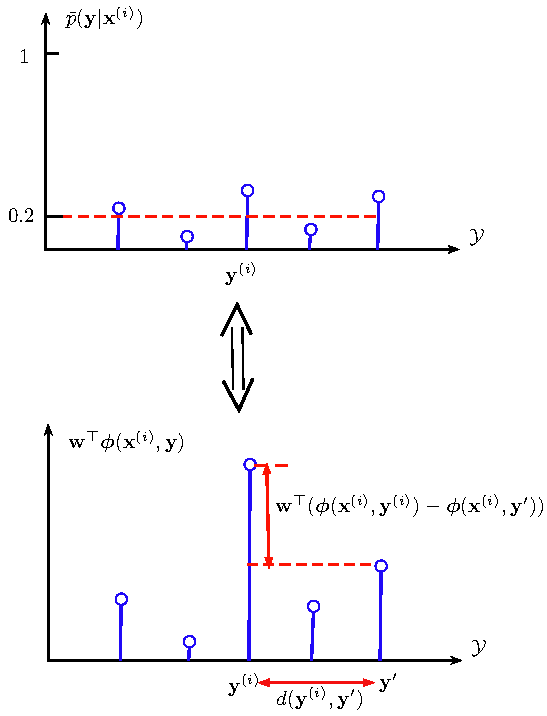
\includegraphics[width=0.49\textwidth]{./Figures/M3N_outputs.pdf}\label{fig:M3N_outputs}}
    \subfigure[]{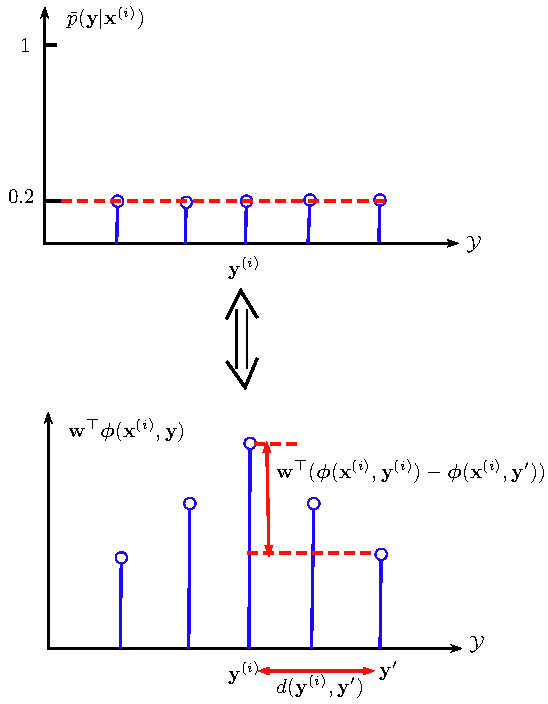
\includegraphics[width=0.49\textwidth]{./Figures/M3N_outputs_smooth.pdf}\label{fig:M3N_outputs_smooth}}
    \caption{Two possible cases  of $p(\mathbf{y}|\mathbf{x}^{(i)})$ and corresponding $\mathbf{w}^\top\boldsymbol{\phi}(\mathbf{x}^{(i)},\mathbf{y})$, when $\mathcal{L}^{Margin}$ is minimized. } 
    \label{fig:M3N_outputs_both}
\end{figure}



\subsubsection{Maximum Entropy within MAP Learning}
For simplicity, at first it is assumed that there exists only one training instance $\{\zeta,t\}$ in $\mathcal{D}$.  
Since $\bar{\mathcal{L}}^{MAP}_\zeta$ is convex, the gradient of minimum point $\mathbf{w}^*$ is 0: 
\begin{equation}
    \left.\frac{d \bar{\mathcal{L}}^{MAP}_\zeta}{d \mathbf{w}}\right|_{\mathbf{w}^*}=\boldsymbol{\phi}(\zeta, t)-\mathbb{E}_{\bar p(\mathbf{y}|\zeta;\mathbf{w}^*)} \left(\boldsymbol{\phi}(\zeta,\mathbf{y})+d(t,\mathbf{y})\right)=0
    \label{equ:equality_1}
\end{equation}
From (\ref{equ:equality_1}), it is not so obvious how l2-norm regularization can affect entropy of $\bar p(\mathbf{y}|\zeta;\mathbf{w}^*)$.    
However, by multiplying $\bar{\mathbf{w}}^{*\top}$ ($\bar{\mathbf{w}}^{*\top}=[\mathbf{w}^{*\top},1]$) on the both sides of (\ref{equ:equality_1}), it becomes: 
\begin{equation}
    \mathbf{w}^{*\top}\boldsymbol{\phi}(\zeta, t)-\mathbb{E}_{\bar p(\mathbf{y}|\zeta; \mathbf{w}^*)} \left(\mathbf{w}^{*\top} \boldsymbol{\phi}(\zeta,\mathbf{y})+d(t,\mathbf{y})\right)=0 
\end{equation}
or equivalently:
\begin{equation}
    \begin{array}{ll}
                   & \mathbf{w}^{*\top}\boldsymbol{\phi}(\zeta, t)=\mathbb{E}_{\bar p(\mathbf{y}|\zeta; \mathbf{w}^*)} \left(\mathbf{w}^{*\top}\boldsymbol{\phi}(\zeta,\mathbf{y})+d(t,\mathbf{y})\right)\\ 
    \Leftrightarrow& \mathbf{w}^{*\top}\boldsymbol{\phi}(\zeta, t)-\log \mathbf{Z}(\bar{\mathbf{w}})= \mathbb{E}_{\bar p(\mathbf{y}|\zeta; \mathbf{w}^*)}(\mathbf{w}^{*\top} \boldsymbol{\phi}(\zeta,\mathbf{y})+d(t,\mathbf{y})-\log \mathbf{Z}(\bar{\mathbf{w}})) \\ 
    \Leftrightarrow& \log \bar p(t|\zeta) = \sum_{\mathbf{y}\in\mathcal{Y}} \bar p(\mathbf{y}|\zeta)\log \bar p(\mathbf{y}|\zeta)=-H(\bar p(\mathbf{y}|\zeta)) 
    %&\Leftrightarrow&\exp(\mathbf{w}^{*\top}\boldsymbol{\phi}(\zeta, t))= \exp(\mathbb{E}_{p(\mathbf{y}|\zeta; \mathbf{w}^*)} \mathbf{w}^{*\top} \boldsymbol{\phi}(\zeta,\mathbf{y}))\\ \\
    %&\Leftrightarrow&\exp(\mathbf{w}^{*\top}\boldsymbol{\phi}(\zeta, t))\leq \mathbf{E}_{p(\mathbf{y}|\zeta; \mathbf{w}^*)} \exp(\mathbf{w}^{*\top} \boldsymbol{\phi}(\zeta,\mathbf{y})) \\ \\ 
    %&\Leftrightarrow&\frac{\exp(\mathbf{w}^{*\top}\boldsymbol{\phi}(\zeta, t))}{\mathbf{Z(\mathbf{w}^*)}}\leq \mathbf{E}_{p(\mathbf{y}|\zeta; \mathbf{w}^*)} \exp(\mathbf{w}^{*\top} \boldsymbol{\phi}(\zeta,\mathbf{y})) \\ \\
    \end{array}
    \label{equ:entropy}
\end{equation}
where $H(\bar p(\mathbf{y}|\zeta))$ denotes the \emph{Shannon's entropy} of $\bar p(\mathbf{y}|\zeta)$. Note that we also have the constraint for the conditional probabilities:   
\begin{equation}
    \sum_{\mathbf{y}\in{\mathcal{Y}}} \bar p(\mathbf{y}|\zeta)=1
    \label{equ:sum_to_1}
\end{equation}
According to (\ref{equ:entropy}) and (\ref{equ:sum_to_1}), there can be two situations. At first, when $\bar p(t|\zeta)$ is big, then the gap between $\bar p(t|\zeta)$ and all other  
$\bar p(\mathbf{y}:\mathbf{y}\in\mathcal{Y}/t|\zeta)$ should be large and different to decrease the entropy (Figure \ref{fig:small_entropy}). Secondly, when $\bar p(t|\zeta)$ is small,       
then to ensure large entropy, all other $\bar p(\mathbf{y}:\mathbf{y}\in\mathcal{Y}/t|\zeta)$ will be similar to each other and close to $\bar p(t|\zeta)$ to increase the 
entropy (Figure \ref{fig:large_entropy}).  
When there are more training instances in $\mathcal{D}$ are considered, the situations are analogous, although mathematics will be more complicated.    
Since $\log \bar p(\mathbf{y}^{(i)}|\mathbf{x}^{(i)})$  
is anti-correlated with $H(\bar p(\mathbf{y}|\mathbf{x}^{(i)}))$.  One simple extra regularization term can be added to bias the MAP solution towards max-entropy:    
\begin{equation}
    \Omega(\mathbf{w})=\sum_{i=1}^M\log \bar p(\mathbf{y}^{(i)}|\mathbf{x}^{(i)})=-\sum_{i=1}^M \bar{\mathcal{L}}^{MAP}_i
\end{equation}
which is actually the log-likelihood of $\mathcal{D}$. Then the resulting objective function is: 
\begin{equation}  
    \mathbf{w}^* =\arg\min_{\mathbf{w}} \frac{1}{2} ||\mathbf{w}||^2+  \frac{C-C_2}{M}\sum_{i=1}^M \bar{\mathcal{L}}^{MAP}_i, \quad C_2\geq0
       \label{equ:MEnMAP}
\end{equation}
which is nothing but reducing the trade-off weight on the mean loss, or equivalently, increasing weight on the l2-norm regularization term, compared to the 
original one.    
Therefore, it can also be claimed that the l2-norm regularization term within MAP learning also performs as an entropy maximizer.  
\begin{figure}[t]
    \centering
    \subfigure[]{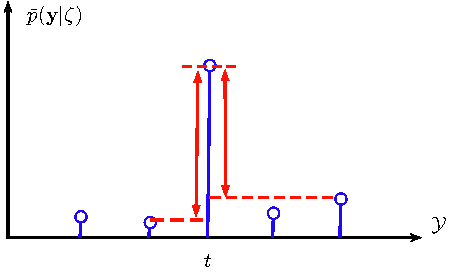
\includegraphics[width=0.48\textwidth]{./Figures/large_margin.pdf}\label{fig:small_entropy}} 
    \subfigure[]{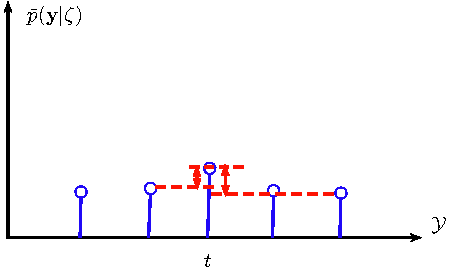
\includegraphics[width=0.48\textwidth]{./Figures/small_margin.pdf}\label{fig:large_entropy}}
    \caption{Two possible cases of $\bar{p}(\mathbf{y}|\zeta)$ when $\bar{\mathcal{L}}^{MAP}$ is minimized.  } 
    \label{fig:MAP_outputs}
\end{figure}


%----------------------------------------------------------------------------------------
%	SECTION 2
%----------------------------------------------------------------------------------------
\section{Training Undirected Graphical Models with Persistent Sequential Monte Carlo}

\begin{shaded}
{\Huge II.} \textbf{Hanchen Xiong}, Sandor Szedmak, Justus Piater. {\it Towards Maximum Likelihood: Learning Undirected Graphical Models using Persistent Sequential Monte Carlo}, The 6th Asian Conference on Machine Learning (ACML2014), 
\end{shaded}
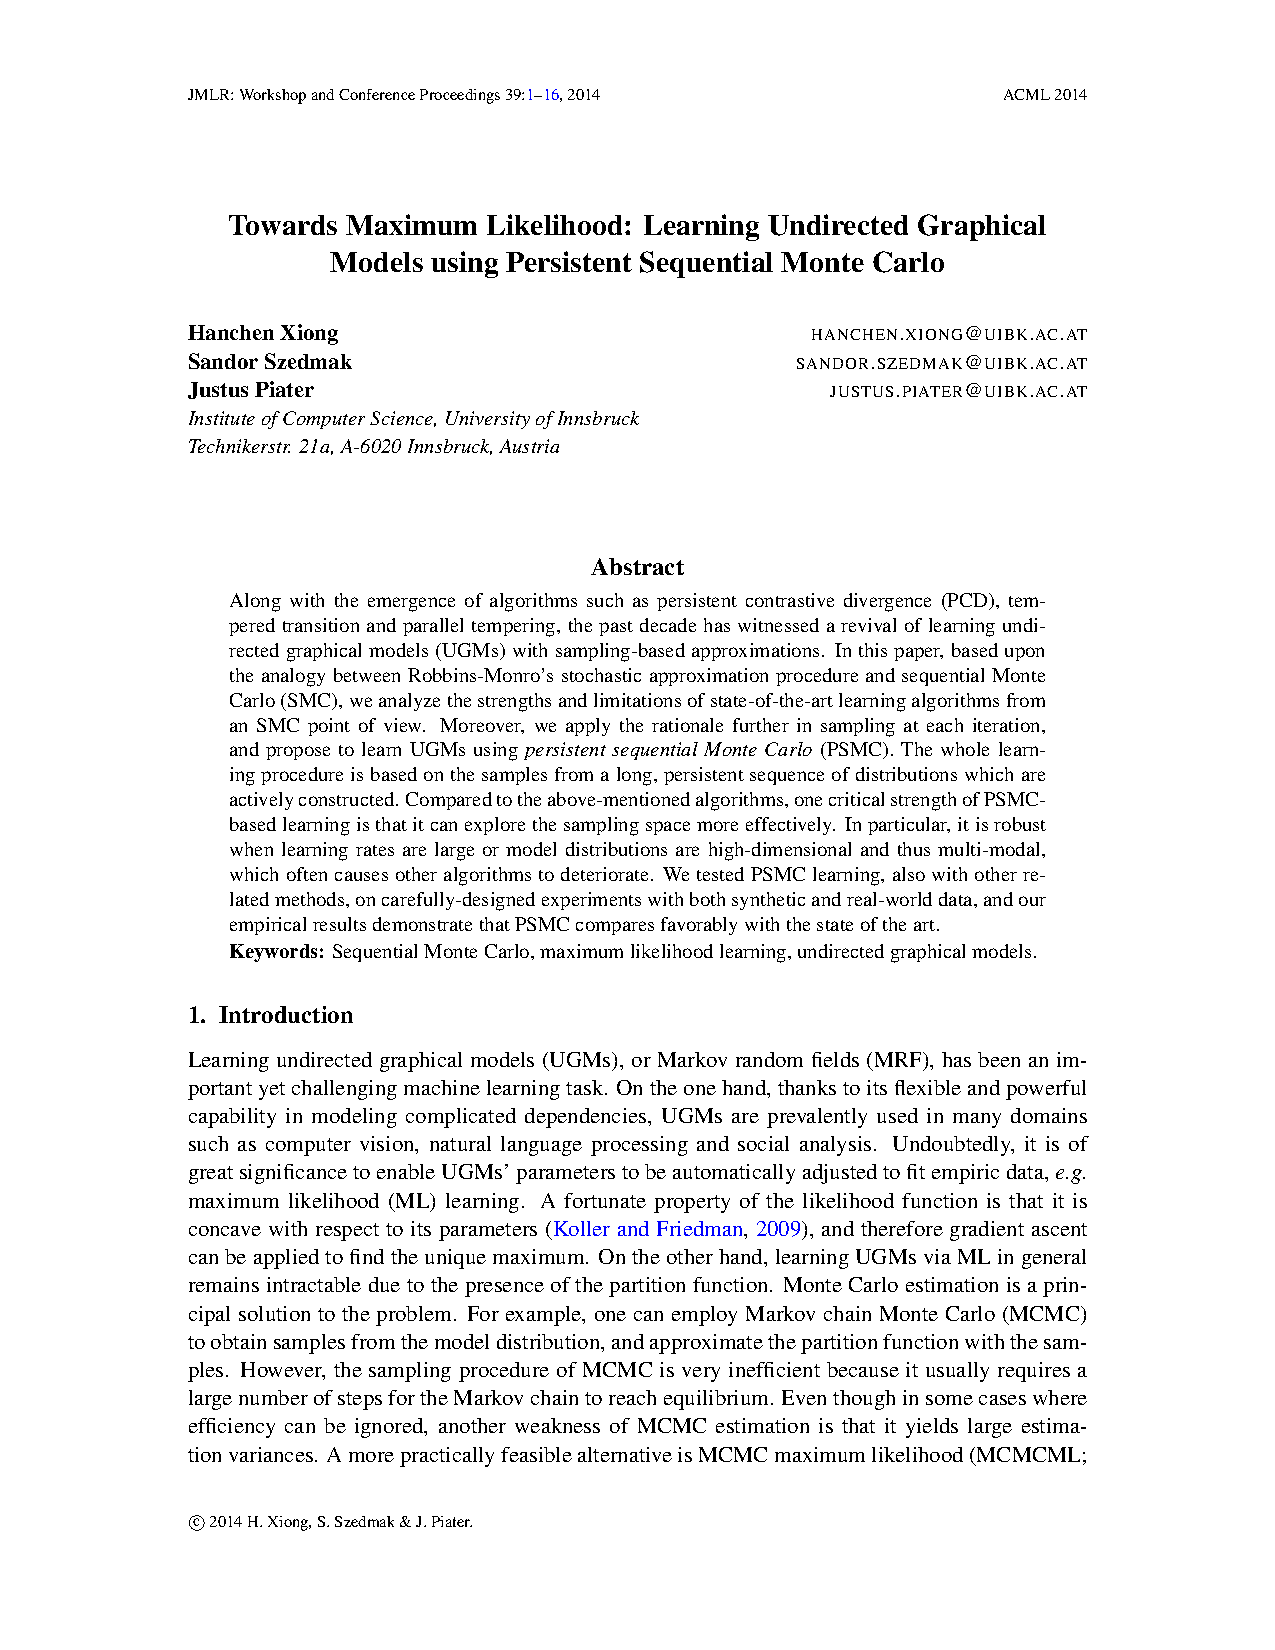
\includepdf[offset=3cm -2.5cm, scale=1, pages=-,pagecommand={\pagestyle{fancy}}]{./Papers/Xiong-2014-ACML.pdf}

\subsection {Training Conditional Random Fields for Image Annotation and Image Segmentation}
In this section we present some evaluations and comparison of different learning algorithms on two practical tasks: \emph{multi-label learning} and \emph{image 
segmentation}. Different from previous experiments where generative models were learned, here we trained discriminative models. Therefore, two 
conditional random fields were employed. Generally speaking, let us denote $\mathbf{x}$ as input and $\mathbf{y}\in \mathcal{Y}$ as output, and our target is to 
learn an UGM:  
\begin{equation}
	p(\mathbf{y}|\mathbf{x})=\frac{\exp(\boldsymbol{\theta}^\top \phi(\mathbf{y},\mathbf{x}))}{\mathbf{Z}}
\end{equation}
where the partition function $\mathbf{Z}$ is
\begin{equation}
	\mathbf{Z}=\sum_{\mathbf{y}\in\mathcal{Y}}\exp(\boldsymbol{\theta}^\top \phi(\mathbf{y},\mathbf{x}))
\end{equation}
where $\phi(\mathbf{y},\mathbf{x})$ is defined based on task-oriented dependency structure. Note that the partition function $\mathbf{Z}$ is computed by 
marginalizing out only $\mathbf{y}$ because our interest is a conditional distribution. Six algorithms 
were implemented: PCD-$H$, PCD-1, PT, TT, SMC and PSMC. Similar setups were used for all algorithms as the previous section.  
Learning rate $\eta_t=\frac{1}{10+0.1*t}$ was used and 100 iterations were run. For each input $\mathbf{x}$, 
the size of particle set $\{ \hat{\mathbf{y}}^{(s)}\}$ is 200.  Similar to other supervised learning schemes, a regularization $\frac{1}{2}||\boldsymbol{\theta}||^2$ 
was added and a trade-off parameters was tunned via $k$ folder cross-validation ($k=4$).  

It is worth mentioning that better results can be expected in both experiments by running more iterations, using better learning rates or exploiting 
feature engineering. However, our purpose here is to compare different learning algorithms under the some conditional instead of defeat state-of-the-art 
results in multi-label learning study and image segmentation study respectively. Therefore, we saved our effort in tunning algorithms and constructing 
sophisticated features. 

\subsubsection{Multi-Label Learning}
In multi-label learning, inter-label dependency is rather critical. Assume that input $\mathbf{x}\in \mathbb{R}^d$ and there are $L$ labels (\emph{i.e.} $\mathbf{y}\in\{-1,+1\}^L$), here we modeled all pairwise dependencies among $L$ labels, and therefore 
the constructed conditional random field is:
\begin{equation}
	p(\mathbf{y}|\mathbf{x})=\frac{\exp(\mathbf{y}^\top\mathbf{W}_E \mathbf{y}+\mathbf{y}^\top \mathbf{W}_v \mathbf{x})}{\mathbf{Z}}
	\label{equ:scene_model}
\end{equation}
where $\mathbf{W}_E\in \mathbb{R}^{L\times L}$ captures pairwise dependencies among $L$ labels while $\mathbf{W}_v\in \mathbb{R}^{L\times d}$ reflects the 
dependencies between input $\mathbf{x}$ and all individual labels.   
In the test phase, with learned $\mathbf{W}_E$ and $\mathbf{W}_v$, for a test input $\mathbf{x}^\dagger$, we predict the corresponding $\mathbf{y}^\dagger$ with 
100 rounds of gibbs sampling based on (\ref{equ:scene_model}).  

In our experiment, we used popular \emph{scene} database \citep{scene_database}, where scene images are associated with a few semantic labels. In the database, 
there are 1121 training instances and 1196 test instances.  In total there are 6 labels ($L=6$) and a 294 dimensional feature were extracted from each image         
($\mathbf{x}\in\mathbb{R}^{294}$). Readers are referred to \cite{scene_database} for more details about the database and feature extraction.  

We evaluated the performance of multi-label learning using \emph{precision} (P), \emph{recall} (R), and the \emph{F1} measure (F). For each label, the precision is 
computed as the ratio of the number of images assigned the label correctly over the total number of images predicted to have the label, while the recall is the number of images 
assigned the label correctly divided by the number of images that truly have the label. Then precision and recall are averaged across all labels. Finally, the F1 measure is calculated as 
$F=2\frac{P\times R}{P+R}$.
The results of all six algorithms are presented in Table \ref{tab:scene_results}.     
The average number temperatures in PSMC is around 5, so PCD-5 was implemented. Also 5 temperatures were use in PT and TT.    
We can see that PSMC yields the best F1 measure 75.1, followed by PT and SMC with 74.6 and 73.4 respectively. The results of PCD-5 and TT             
are relative worse, while PCD-1 is the worst.  


\begin{table}
	\label{tab:scene_results}
	\center
\begin{tabular}{cccc} 
\Xhline{2\arrayrulewidth} \\ 
       & Precision($\%$) & Recall($\%$) & F1($\%$) \\ \hline 
 PCD-1 & 57.7            & 59.3         & 58.5 \\
 PCD-5 & 70.3            & 72.6         & 71.4 \\
 TT    & 70.0            & 67.5         & 68.7 \\
 PT    & {\bf 72.2}      & 77.1         & 74.6 \\
SMC    & 71.7            & 75.1         & 73.4 \\
PSMC   & 71.9            & {\bf 78.5}   & {\bf 75.1} \\ 
\Xhline{2\arrayrulewidth}
 \end{tabular}
 \caption{A comparison of six learning algorithms on multi-label learning. }
\end{table}

\subsubsection{Image Segmentation} 
Image segmentation essentially is a task to predict the semantic label of all image pixels or blocks.    
Inter-label dependences within neighbourhood are usually exploited in image segmentation. For instance, by dividing an image into equal size and non-overlapping 
blocks, the label of a block does not only depend on the appearance of the block, but also the labels of its neighbouring blocks. For simplicity, here 
we only consider binary labels. In addition, we assume that blocks and inter-label dependencies are position irrelevant. Therefore, a conditional random filed can 
be constructed as:               
\begin{equation}
	p(\mathbf{y}|\mathbf{x})=\frac{\exp(\sum_{u,v\in E}y_u W_e y_v+\sum_{v\in V} y_v \mathbf{w}_v^\top \mathbf{x}_v) }{\mathbf{Z}}
\end{equation}
where $y_v\in\{-1,+1\}$, $E$ denotes the set of all edges connecting neighbouring blocks, $W_e\in\mathbb{R}$ encodes the dependency between neighbouring labels, $V$ denotes the set of all 
block's labels and $\mathbf{w}_v\in \mathbb{R}^{d\times 1}$ encodes the dependency between block label and its appearance which is represented by a $d$-dimensional feature $\mathbf{x}_v\in\mathbb{R}^d$.    
Similar to the multi-label experiment, desired labels are predicted via 100 round gibbs sampling in test phase.      

In our experiment, we used the binary segmentation database from \cite{img_seg_database}, where each image is divided into non-overlapping blocks of 
size $16\times16$ and each block is annotated with either ``man-made structure" (MS) or ``nature structure" (NS). 
Overall, there are 108 training images and 129 test images. The training set contains 3004 MS blocks and 36269 NS blocks, while the test set 
contains 6372 MS blocks and 43164 NS blocks.
For each block, its appearance is 
represented by a 3-dimensional features which includes the mean of gradient magnitude, the 'spikeness' of the count-weighted histogram of gradient orientations, 
the angle between the most frequent orientation and the second most frequent orientation. The feature was designed to fit this specific application.        
More explanation of the database and feature design can be found in \cite{img_seg_database}. 


We found that the average number of temperatures in PSMC is 20, therefore PCD-20 was run and 20 temperatures were used in TT and PT. We quantify the segmentation performance of 
six algorithms with confusion matrices, which are presented in Figure \ref{fig:img_seg_results}. We can see that PSMC outperforms all others (by checking the diagonal entries of confusion matrices).      
For qualitative comparison, an example image and corresponding segmentations are shown in Figure \ref{fig:img_seg_example}.  It can be seen that the segmentation by PSMC is closer to the ground truth 
compared to others. 
\begin{figure}[t!] 
    \centering
    \subfigure{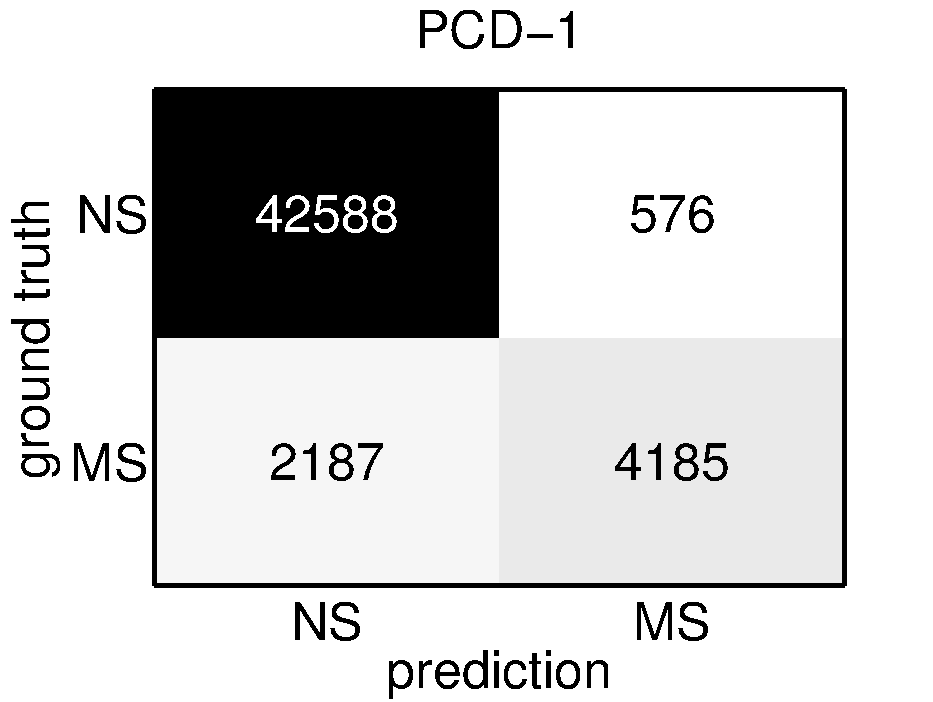
\includegraphics[width=0.48\textwidth]{./Figures/CM_PCD_1}\label{fig:CM_PCD_1}}
    \subfigure{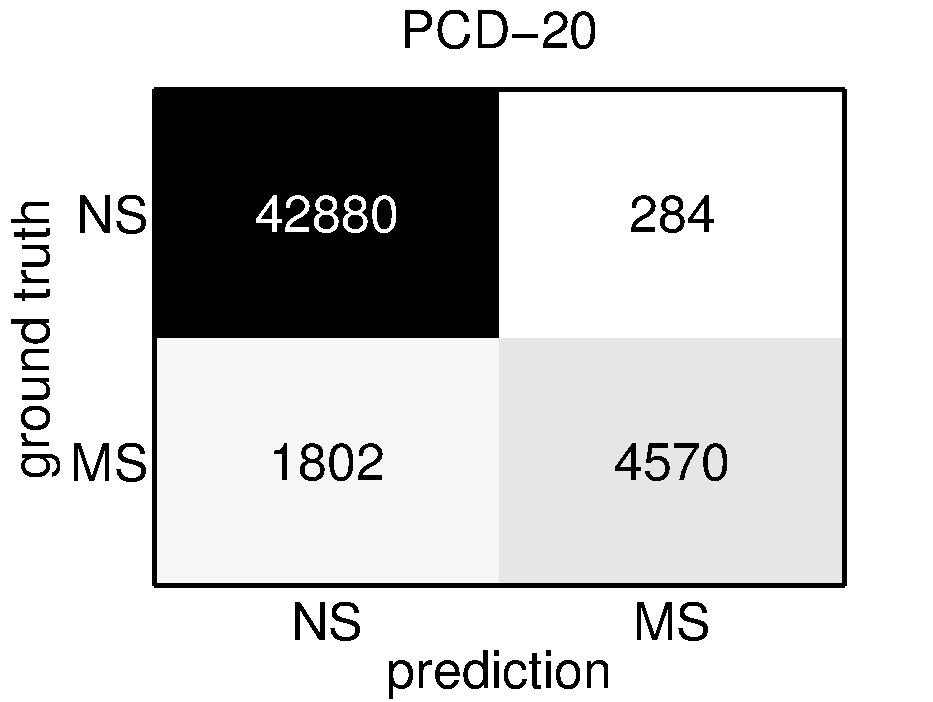
\includegraphics[width=0.48\textwidth]{./Figures/CM_PCD_20}\label{fig:CM_PCD_20}}
	\subfigure{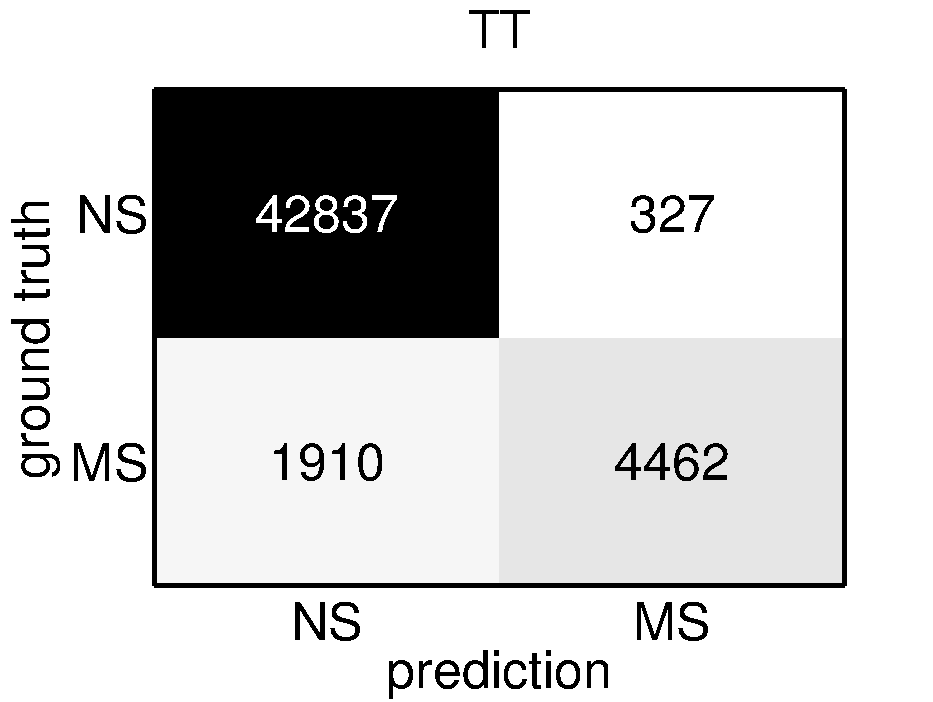
\includegraphics[width=0.48\textwidth]{./Figures/CM_TT}\label{fig:CM_TT}}
	\subfigure{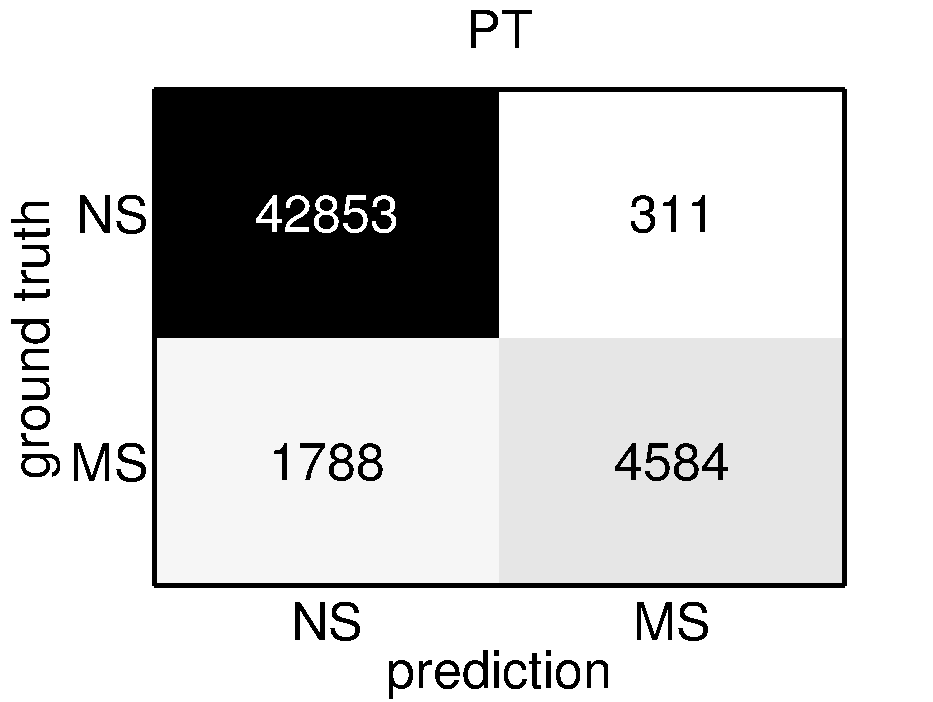
\includegraphics[width=0.48\textwidth]{./Figures/CM_PT}\label{fig:CM_PT}}
	\subfigure{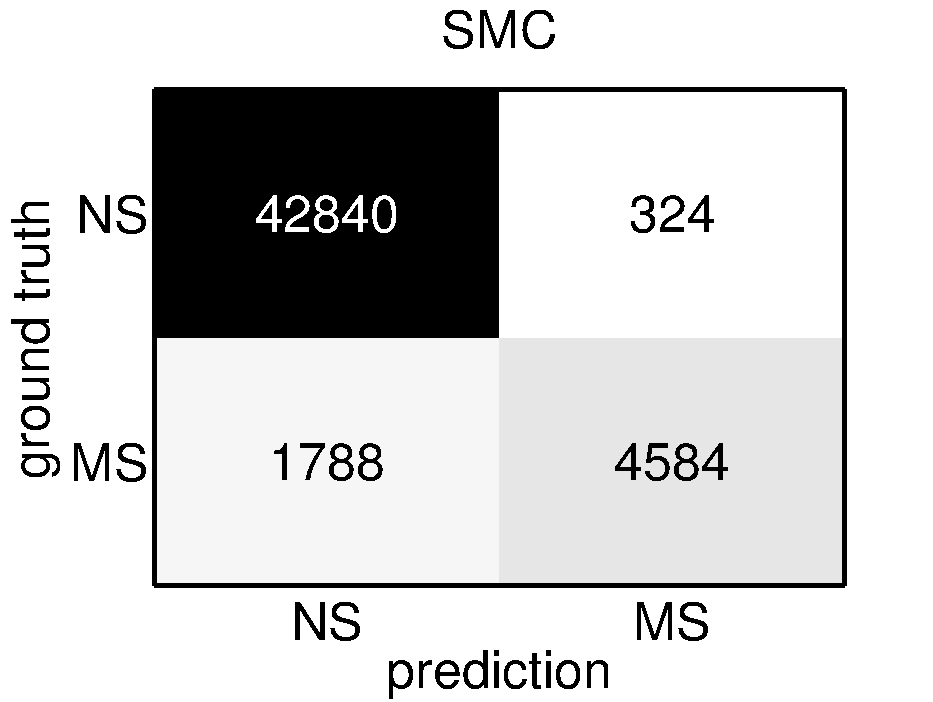
\includegraphics[width=0.48\textwidth]{./Figures/CM_SMC}\label{fig:CM_SMC}}
	\subfigure{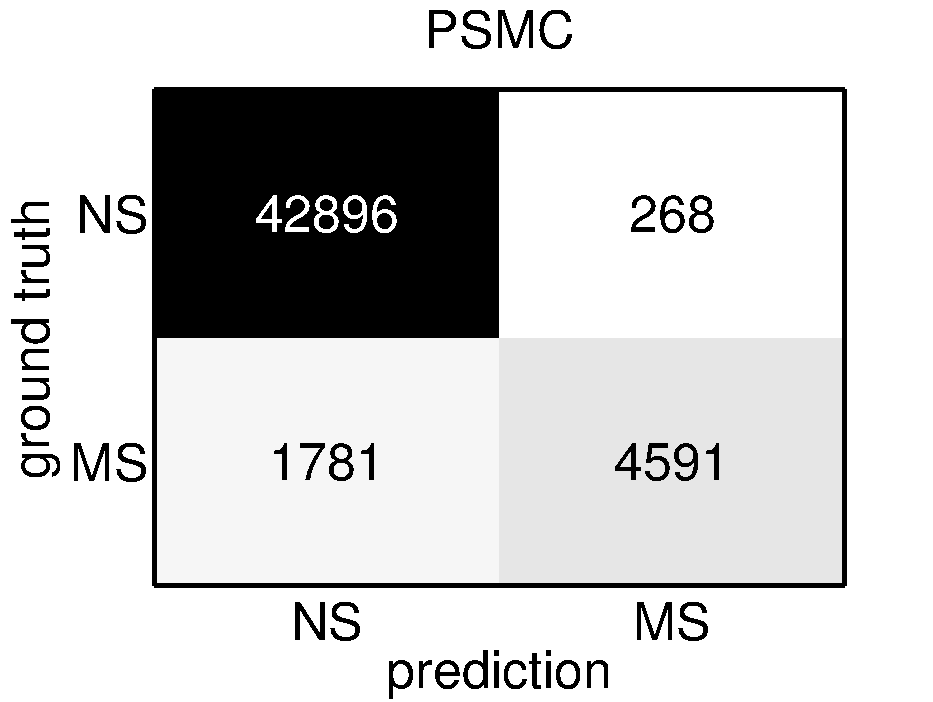
\includegraphics[width=0.48\textwidth]{./Figures/CM_PSMC}\label{fig:CM_PSCM}}
    \caption{Confusion matrices of binary segmentation by six algorithms.}   
    \label{fig:img_seg_results}
\end{figure}

\begin{figure}[t!] 
    \centering
    \subfigure[]{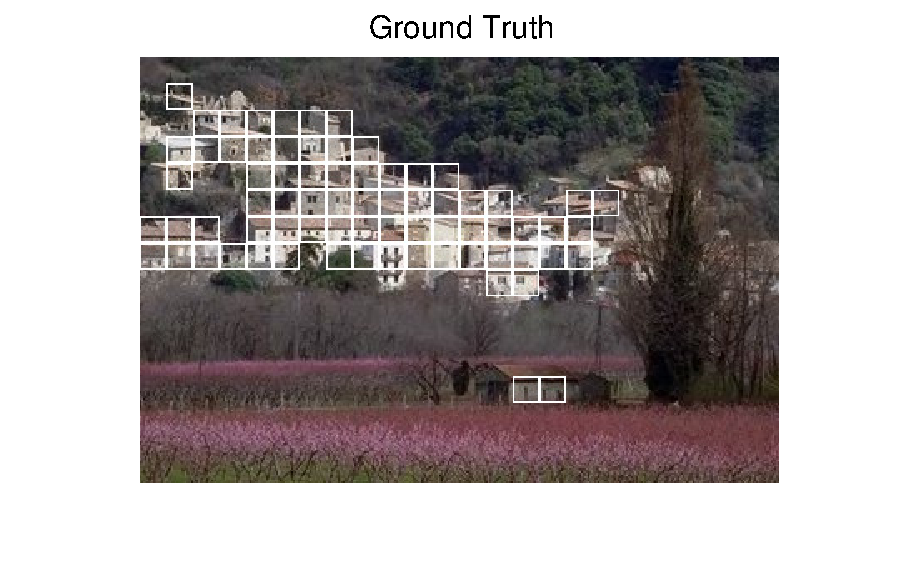
\includegraphics[width=0.7\textwidth]{./Figures/img_seg_GT}\label{fig:img_seg_GT}} \\
    \subfigure[]{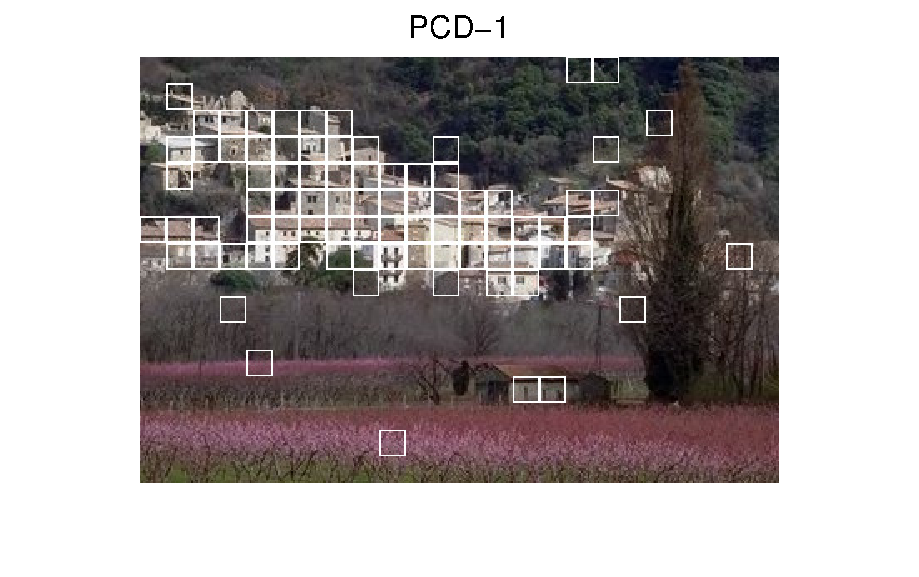
\includegraphics[width=0.49\textwidth]{./Figures/img_seg_PCD_1}\label{fig:img_seg_PCD_1}}
    \subfigure[]{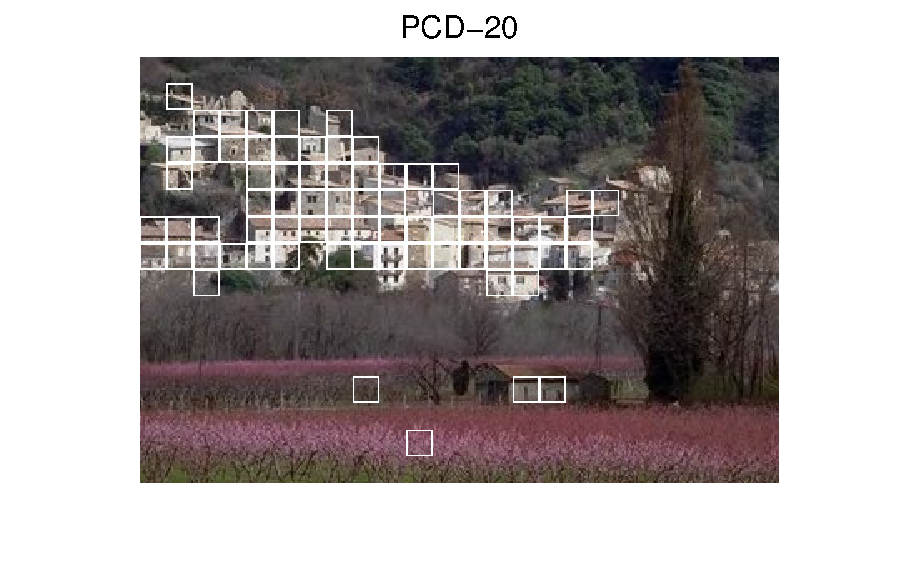
\includegraphics[width=0.49\textwidth]{./Figures/img_seg_PCD_20}\label{fig:img_seg_PCD_20}}
	\subfigure[]{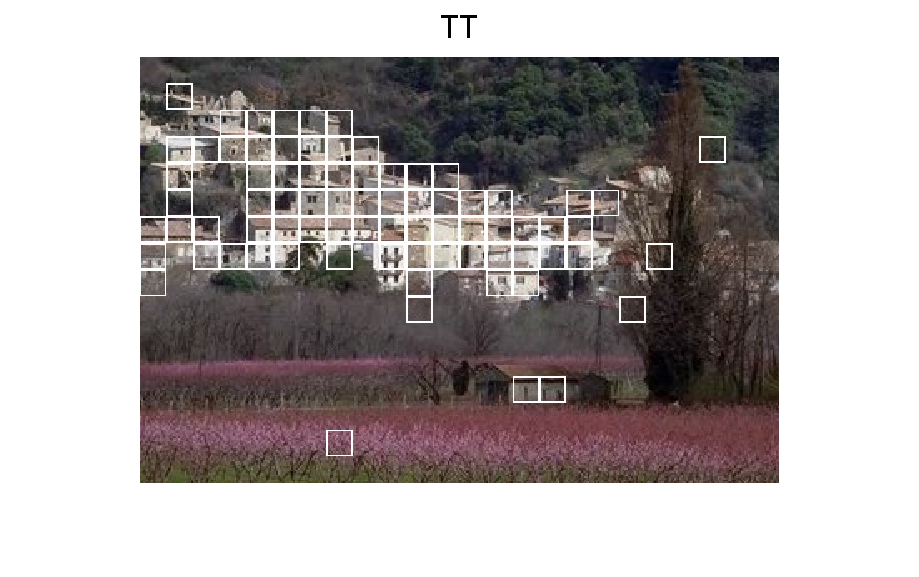
\includegraphics[width=0.49\textwidth]{./Figures/img_seg_TT}\label{fig:img_seg_TT}}
	\subfigure[]{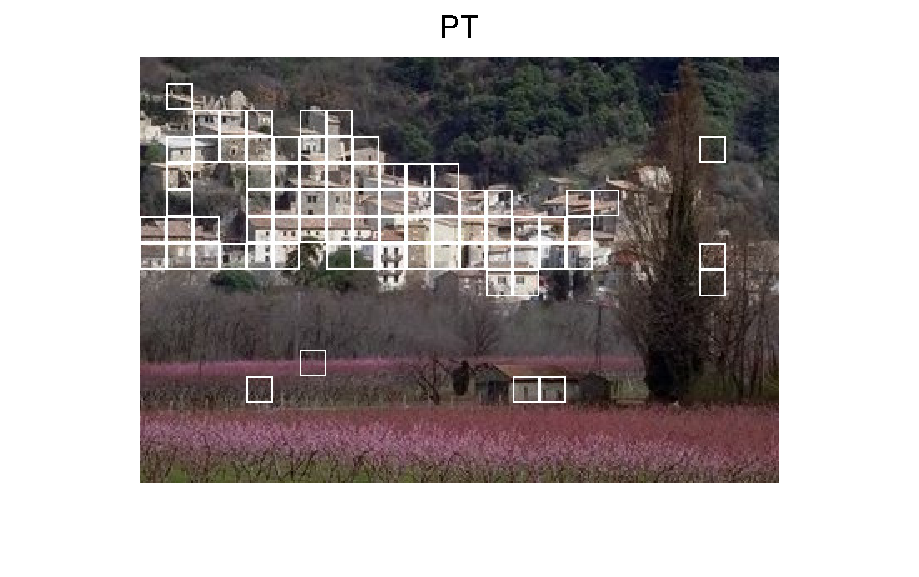
\includegraphics[width=0.49\textwidth]{./Figures/img_seg_PT}\label{fig:img_seg_PT}}
	\subfigure[]{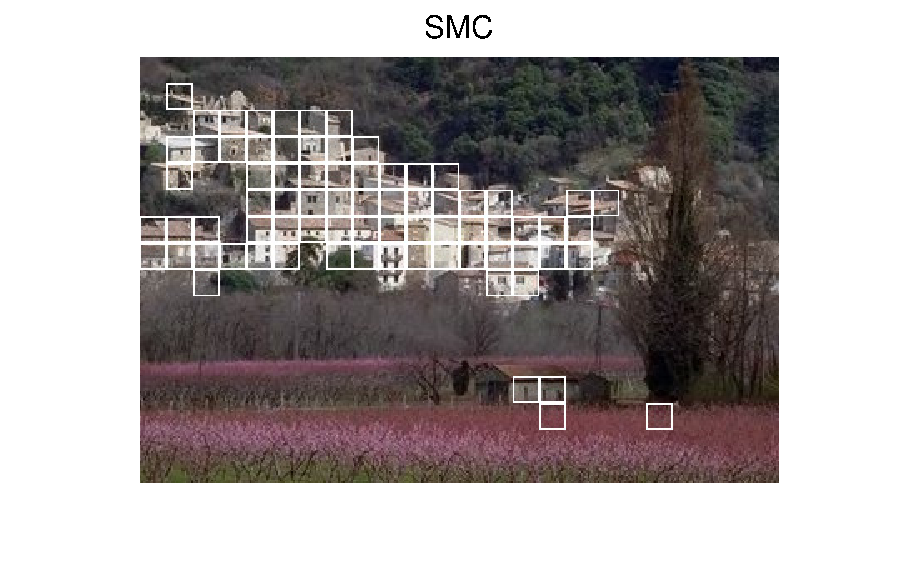
\includegraphics[width=0.49\textwidth]{./Figures/img_seg_SMC}\label{fig:img_seg_SMC}}
	\subfigure[]{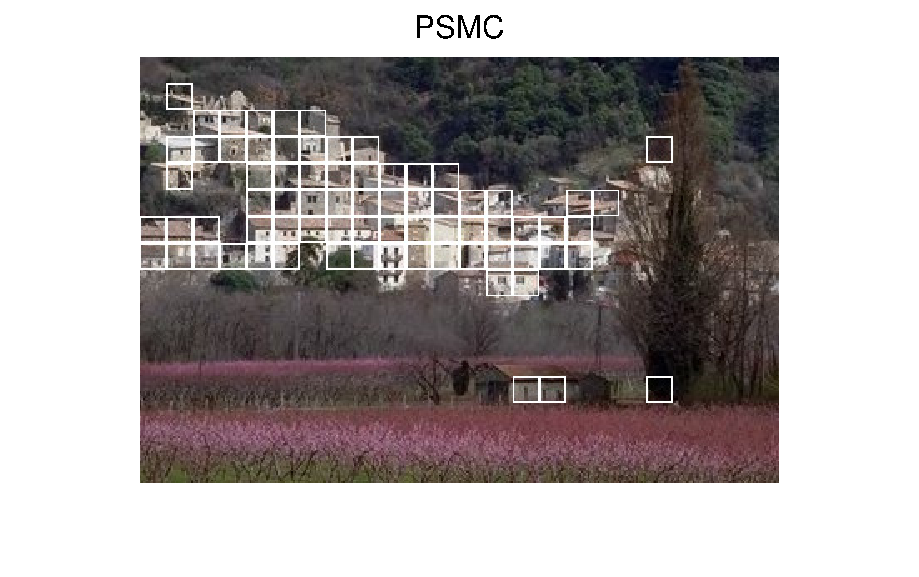
\includegraphics[width=0.49\textwidth]{./Figures/img_seg_PSMC}\label{fig:img_seg_PSCM}}
    \caption{An example image and corresponding segmentations by six algorithms.  }   
    \label{fig:img_seg_example}
\end{figure}



% Chapter Template

\chapter{Kernel-Based Structural Output Learning} % Main chapter title
\label{Chapter4} % Change X to a consecutive number; for referencing this chapter elsewhere, use \ref{ChapterX}
\lhead{Chapter 4. \emph{Kernel-Based Structural Output Learning}} % Change X to a consecutive number; this is for the header on each page - perhaps a shortened title

\rule{\textwidth}{0.4pt} \\[0.5cm]
\textit{``Nothing is more practical than a good theory."}

\begin{flushright}
Vladimir Vapnik
\end{flushright}
\rule{\textwidth}{0.4pt} 


%----------------------------------------------------------------------------------------
%	SECTION 1
%----------------------------------------------------------------------------------------

\section{Joint SVM}

%-----------------------------------
%	SUBSECTION 1
%-----------------------------------
\subsection{Structural SVM for Multi-Label Learning}
\label{subsec:SSVM}
This subsection will introduce structural SVM based on standard SVM and study its application 
in multi-label learning. 
Standard SVM is a binary classifier, which has been well 
understand and widely used in many applications.  
Its two advantageous components are \emph{maximum margins} and \emph{input kernels}. 
The maximum-margin principle is a reflection of statistical learning theory \citep{Vapnik} on 
linear binary classification. 
Kernels provide powerful mechanisms enabling the linear classifier to separate highly non-linear data. 
The critical observation of kernel methods is that a kernel function can be defined on a pair of data 
instances to implicitly map them to a \emph{reproducing kernel Hilbert space} (RKHS):   
\begin{equation}
    K_\phi(\mathbf{x}^{(i)},\mathbf{x}^{(j)})=\langle \phi(\mathbf{x}^{(i)}),\phi(\mathbf{x}^{(j)}) \rangle
 \label{equ:kernel_trick}
\end{equation}
where $\mathbf{x}^{(i)}, \mathbf{x}^{(j)}\in\mathbb{R}^d$ are two input training instances, $\phi$ is the feature map induced by kernel function $K_\phi$, and $\phi(\mathbf{x}^{(i)})$ is the 
representation of 
$\mathbf{x}^{(i)}$ in the RKHS $\mathcal{H}_\phi$.
Given the training dataset $\{\mathbf{x}^{(i)}\in\mathbb{R}^d,y^{(i)}\in\{+1,-1\}\}_{i=1}^m$, the primal form of training SVM is:
\begin{equation}
\begin{array}{rl} 
    \displaystyle \arg\min_{ \mathbf{w} \in \mathbb{R}^{\mathcal{H_{\phi}}}}   & \frac{1}{2} ||\mathbf{w}||^2+C\sum_{i=1}^m \xi^{(i)} \\
    \text{s.t.} & y^{(i)} \left(\mathbf{w}^\top \phi (\mathbf{x}^{(i)})\right) \geq 1-\xi^{(i)}, \xi^{(i)} \geq 0,  i\in \{1,\dots,m\}
\end{array}
\label{equ:hard_svm}
\end{equation}
where $\mathbf{w}$ is a linear hyperplane in $\mathcal{H}_\phi$, $\xi^{(i)}$ are slack variables for the tolerance of noise, and $C$ is a trade-off parameter. 
(\ref{equ:hard_svm}) differs from usual SVM formulation slightly at the absence of a bias term. Here we ignore the bias since 
it can be absorbed in $\mathbf{w}$. 
\footnote{When a Polynomial kernel is used, a bias term is already in its corresponding feature map. When a Gaussian kernel is used, an input vector can be 
augmented with one extra constant.}


\begin{figure}[t]
	\includegraphics[width=\textwidth]{./Figures/SVM_prime}	
	\caption{Understanding the primal form of SVM.}
\end{figure}


Here, to make the transition from SVM to structural SVM more smooth. An alternative interpretaion  
of the primal form of SVM is presented. 
At first, denote $y^{(i)} \left(\mathbf{w}^\top \phi (\mathbf{x}^{(i)})\right)$ in the constraints of (\ref{equ:hard_svm}) as a score function $F(\mathbf{x}^{(i)},y^{(i)}; \mathbf{w})$, then  
for binary outputs $y^{(i)}$, $F\left(\mathbf{x}^{(i)},y^{(i)}; \mathbf{w}\right)- F\left(\mathbf{x}^{(i)},-y^{(i)}; \mathbf{w}\right)=2\times F\left(\mathbf{x}^{(i)}),y^{(i)}; \mathbf{w}\right)$. 
Also, a distance function between binary outputs can be denoted as $d(y^{(i)},-y^{(i)})=|y^{(i)}-(-y^{(i)})|=2$. Then by replacing $C$ with $\frac{C}{2}$, (\ref{equ:hard_svm}) can be rewritten 
as:
\begin{equation}
\begin{array}{rl}
\displaystyle \arg\min_{ \mathbf{w} \in \mathbb{R}^{\mathcal{H_{\phi}}}}   & \frac{1}{2} ||\mathbf{w}||^2+C\sum_{i=1}^m \xi^{(i)} \\
                                                                       \text{s.t.} & \forall i, F\left(\mathbf{x}^{(i)},y^{(i)}; \mathbf{w}\right)- F\left(\mathbf{x}^{(i)},-y^{(i)}; \mathbf{w}\right) \geq d(y^{(i)},-y^{(i)})-\xi^{(i)}, \xi^{(i)} \geq 0 
\end{array}
\label{equ:binary_SSVM}
\end{equation}
A structural SVM is a simple extension of (\ref{equ:binary_SSVM}) by considering more general $y$. 
Assume that the structural output $\mathbf{y}\in\mathcal{Y}$ and $|\mathcal{Y}|$ is more than 
two. Similarly, a score function can be introduced on a pair of input and output based on the 
nature of the task: $F(\mathbf{x},\mathbf{y};\boldsymbol{\theta})$ where $\boldsymbol{\theta}$ is
a parameter set. Then the primal form of the structural SVM can be   
\begin{equation}
\begin{array}{rl}
\displaystyle \arg\min_{ \mathbf{w} \in \mathbb{R}^{\mathcal{H_{\phi}}}}   & \frac{1}{2} ||\mathbf{w}||^2+C\sum_{i=1}^m \xi^{(i)} \\
                                                                       \text{s.t.} & \forall i, \underbrace{F\left(\mathbf{x}^{(i)},y^{(i)}; \mathbf{w}\right)- F\left(\mathbf{x}^{(i)},-y^{(i)}; \mathbf{w}\right)}_{\Delta_F(y^{(i)},-y^{(i)})} \geq d(y^{(i)},-y^{(i)})-\xi^{(i)}, \xi^{(i)} \geq 0 
\end{array}
\label{equ:binary_SSVM}
\end{equation}

\subsection{Joint SVM: Output Kernel Learning and Regularization }

Joint SVM was developed with a special focus on the interdependencies within outputs in multi-label learning.
Essentially, Joint SVM is equivalent to SSVM with a linear output kernel plus an regularization on the kernel.  
Therefore, a linear kernel on outputs is automatically learned to capture the interdependencies within outputs.  
Furthermore, if prior knowledge about the interdependencies is available, a user-specified output kernel can be 
straightforwardly mounted in Joint SVM as well.  
In both cases, the computation complexity of Joint SVM is almost the same as a single SVM, in contrary to the 
exponential complexity in structural SVM. 
Joint SVM was shown to yield substantial
improvements, in terms of both accuracy and efficiency, over
training them independently. In particular, it outperforms many
other state-of-the-art algorithms according to empirical results
on an image-annotation benchmark database. 

More technique detials and results are presented in the paper I and paper III by the author. 
\begin{shaded}
{\Huge I.} \textbf{Hanchen Xiong}, Sandor Szedmak, Justus Piater. {\it Implicit Learning of Simpler Output Kernels for Multi-Lable Prediction}, NIPS workshop on Representation and Learning Methods for Complex Outputs (NIPS-RLCO2014).  
\vspace{-.2cm}

{\Huge III.} \textbf{Hanchen Xiong}, Sandor Szedmak, Justus Piater. {\it Scalable, Accurate Image Annotation with Joint SVMs and Output Kernels}, Neurocomputing Journal (Accepted).  
\vspace{-.2cm}
\end{shaded}



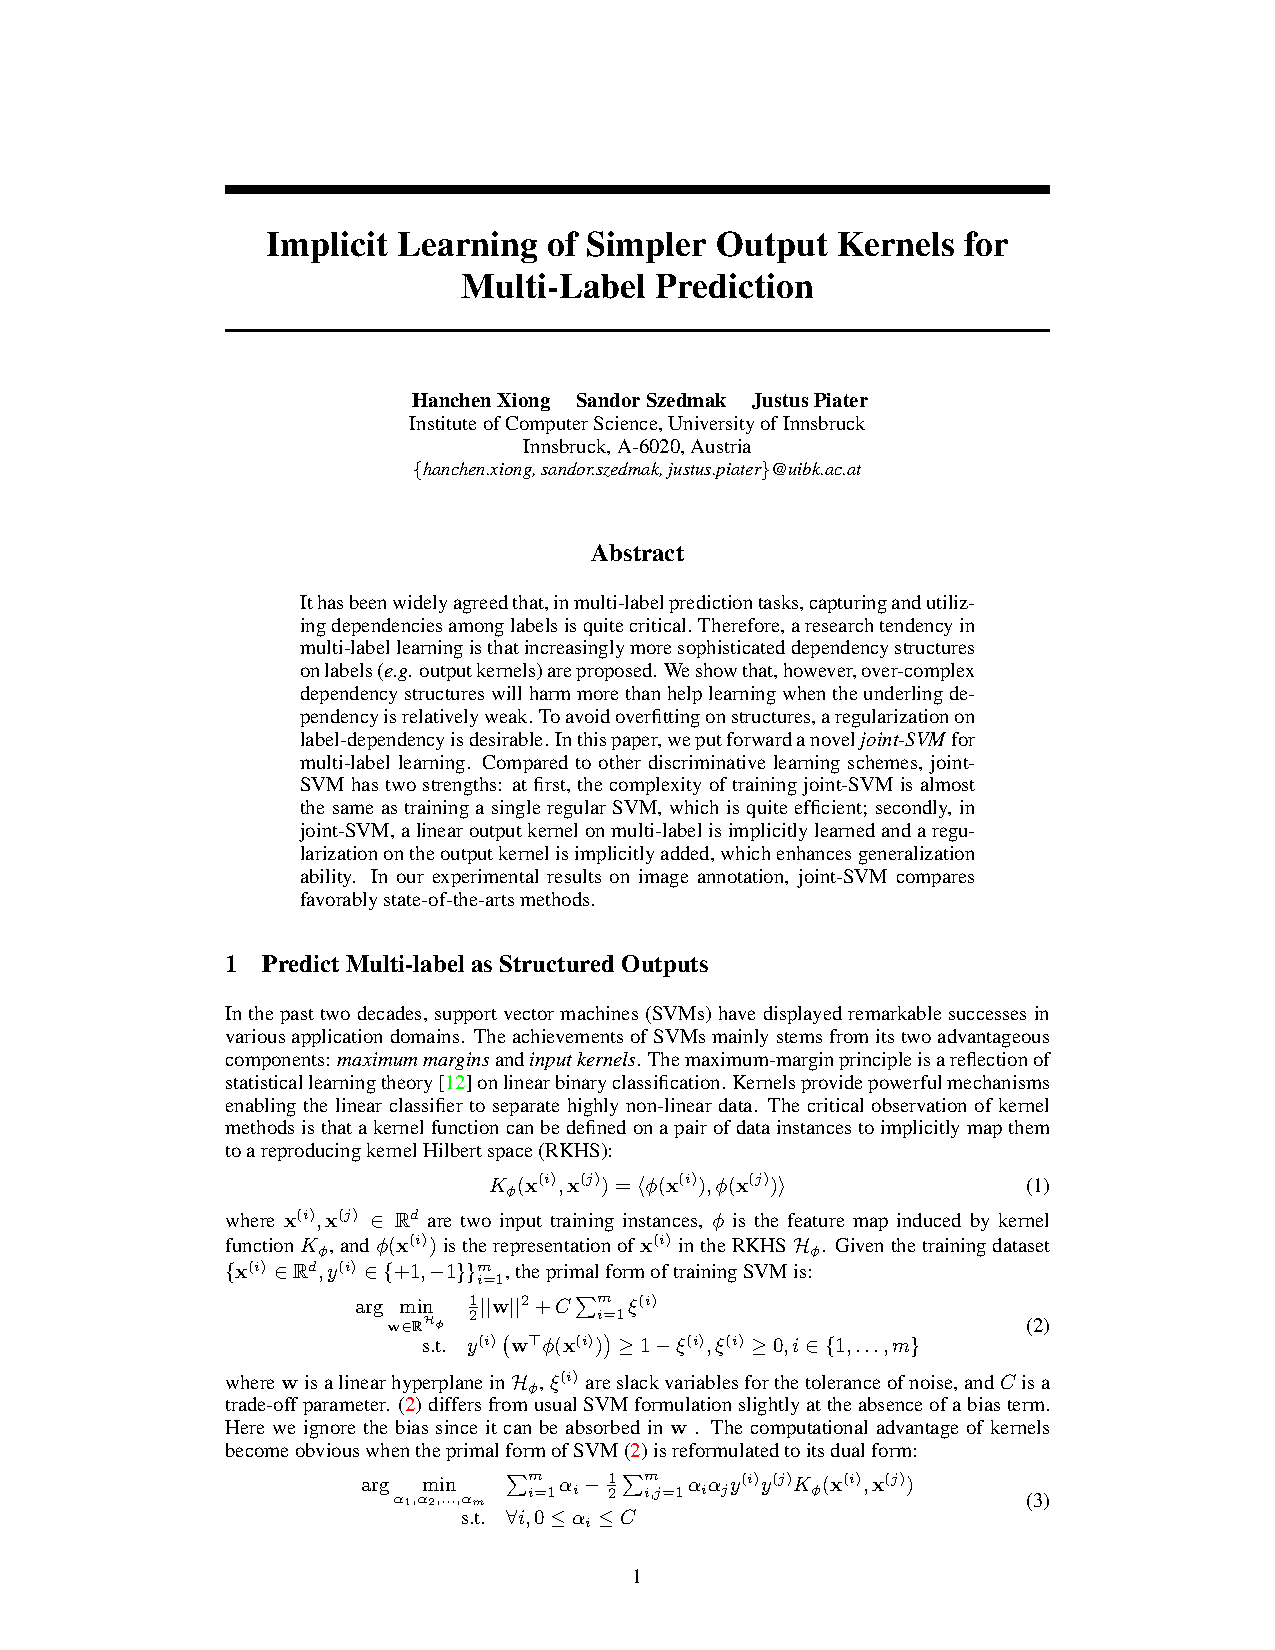
\includepdf[offset=3cm -2cm, scale=1, pages=-,pagecommand={\pagestyle{fancy}}]{./Papers/Xiong-2014-NIPS-RLCO.pdf}
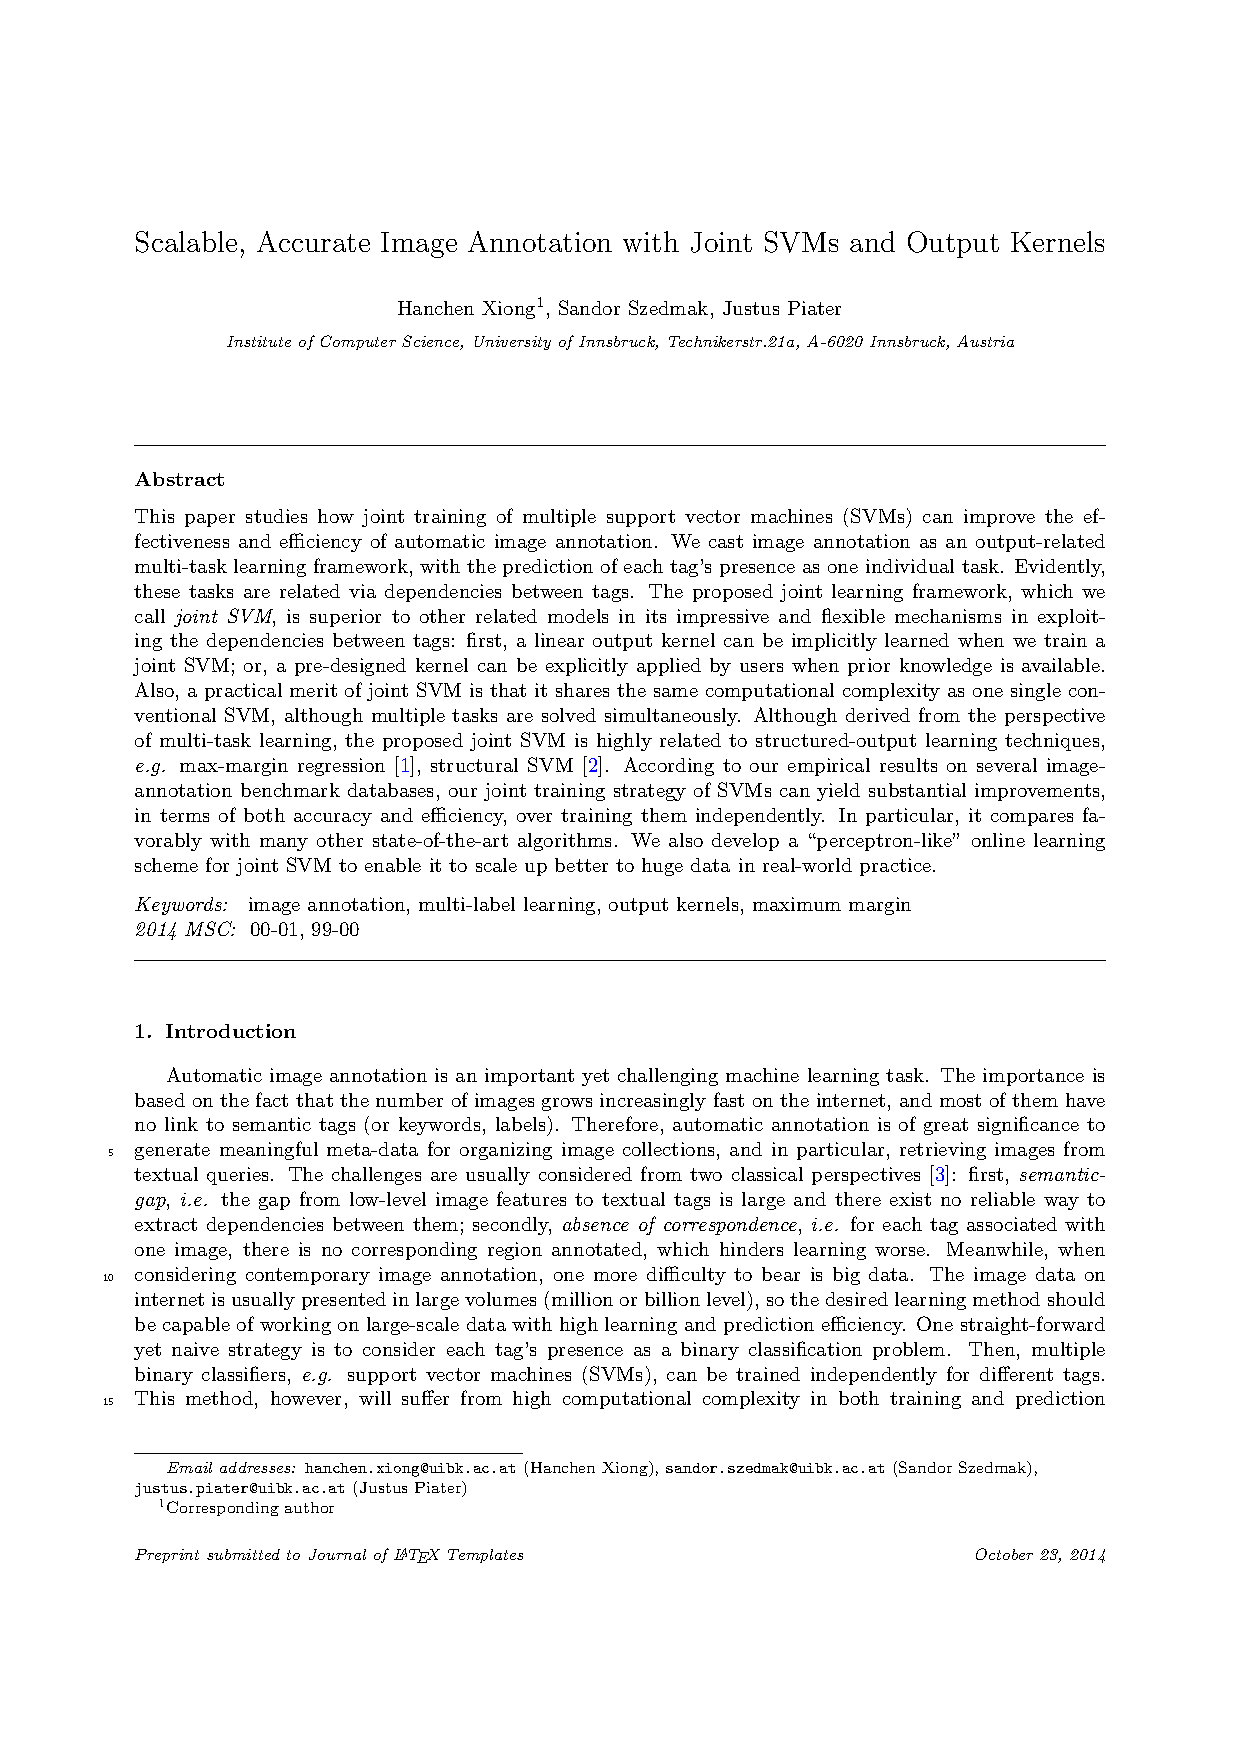
\includepdf[offset=3cm -2cm, scale=1, pages=-,pagecommand={\pagestyle{fancy}}]{./Papers/Xiong-2015-NEUCOM.pdf}





%----------------------------------------------------------------------------------------
%	SECTION 2
%----------------------------------------------------------------------------------------
\section{Homogeneity Analysis for Object-Action Relation Learning}
\begin{shaded}
{\Huge VII.} \textbf{Hanchen Xiong}, Sandor Szedmak, Justus Piater {\it Homogeneity Analysis for Object-Action Relations Reasoning in Kitchen Scenarios}, 
In Proceedings of 2nd Workshop on Machine Learning for Intelligent Systems (MLIS13), pp 37-44,  2013, ACM. 
\vspace{-.2cm}
\end{shaded}

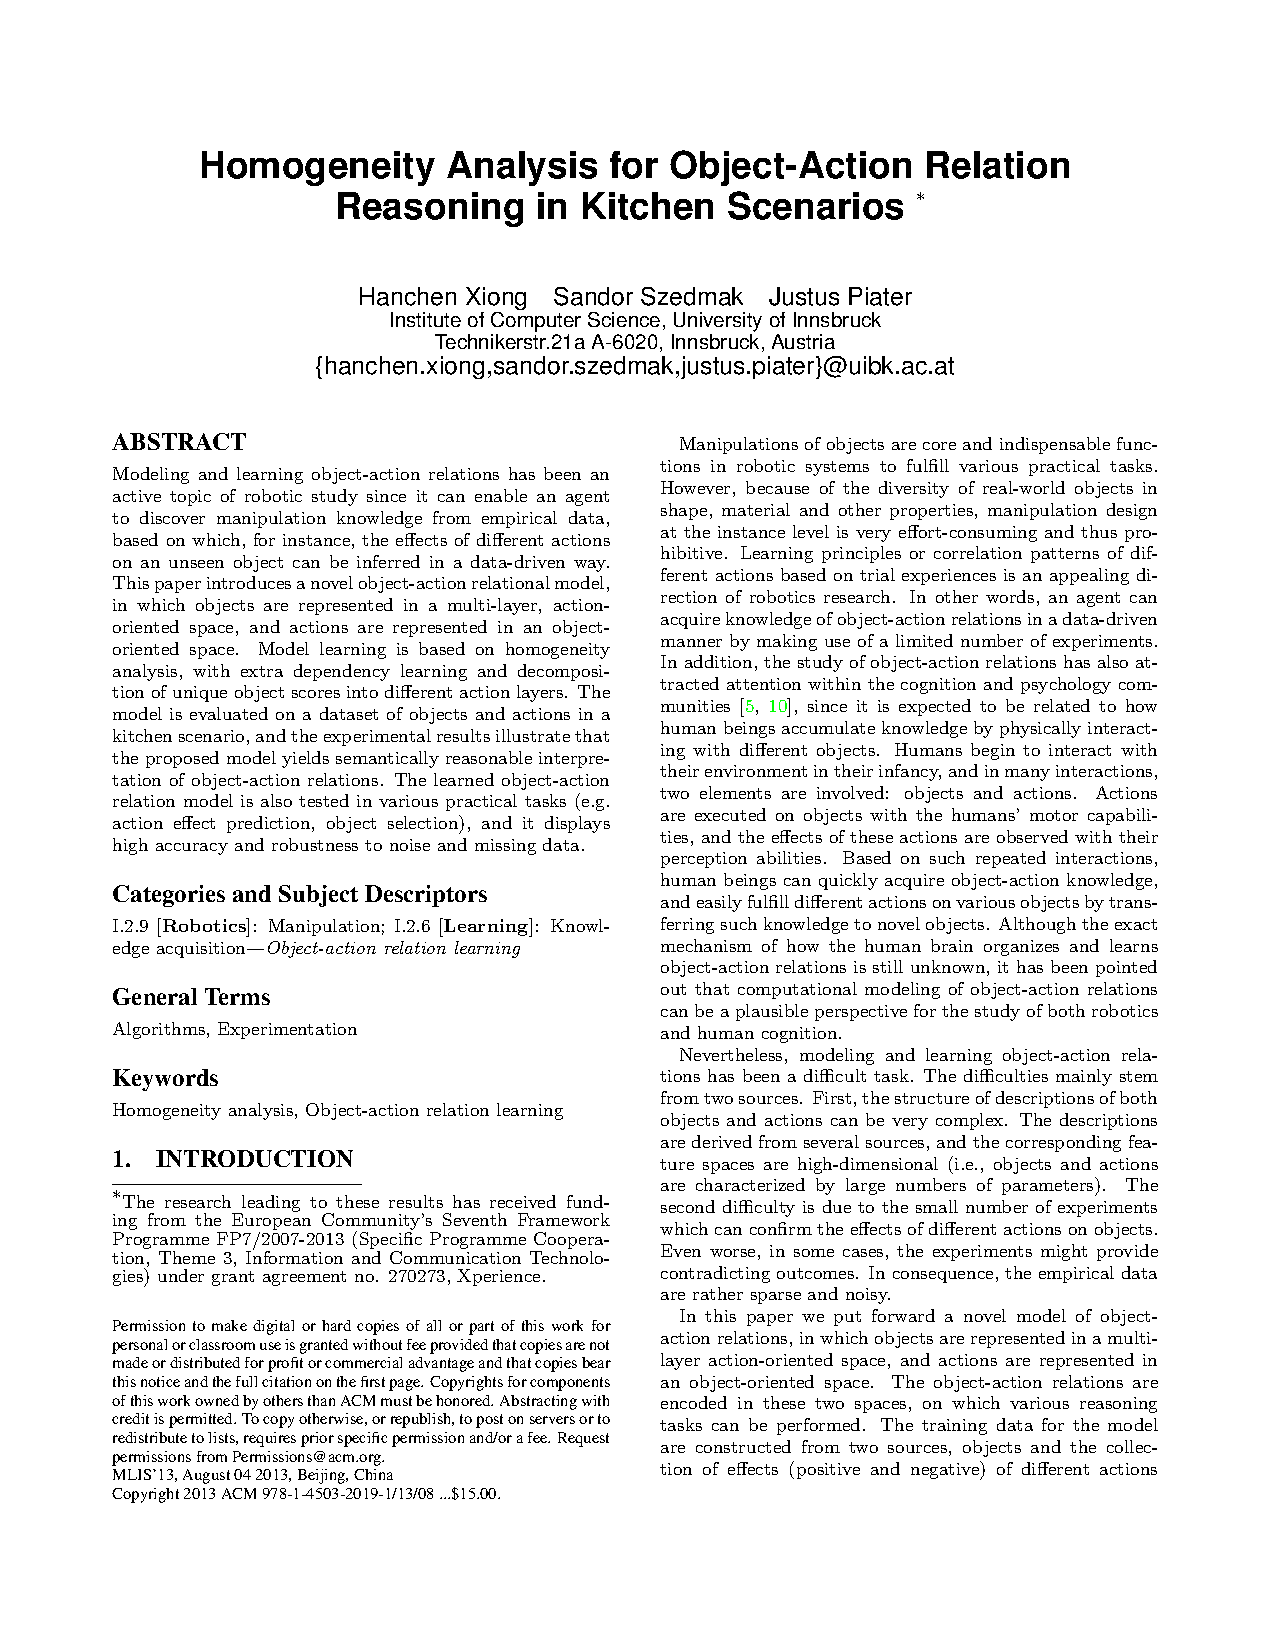
\includepdf[offset=3cm -3cm, scale=1, pages=-,pagecommand={\pagestyle{fancy}}]{./Papers/Xiong-2013-MLIS.pdf}

%----------------------------------------------------------------------------------------
%	SECTION 3
%----------------------------------------------------------------------------------------

\section{Multi-Label Learning with Kernel Generalized Homogeneity Analysis}
\begin{shaded}
 {\Huge X.} \textbf{Hanchen Xiong}, Sandor Szedmak, Justus Piater {\it Multi-Label Learning with Kernel Generalized Homogeneity Analysis}, 
Unpublished, 2015.
\end{shaded}

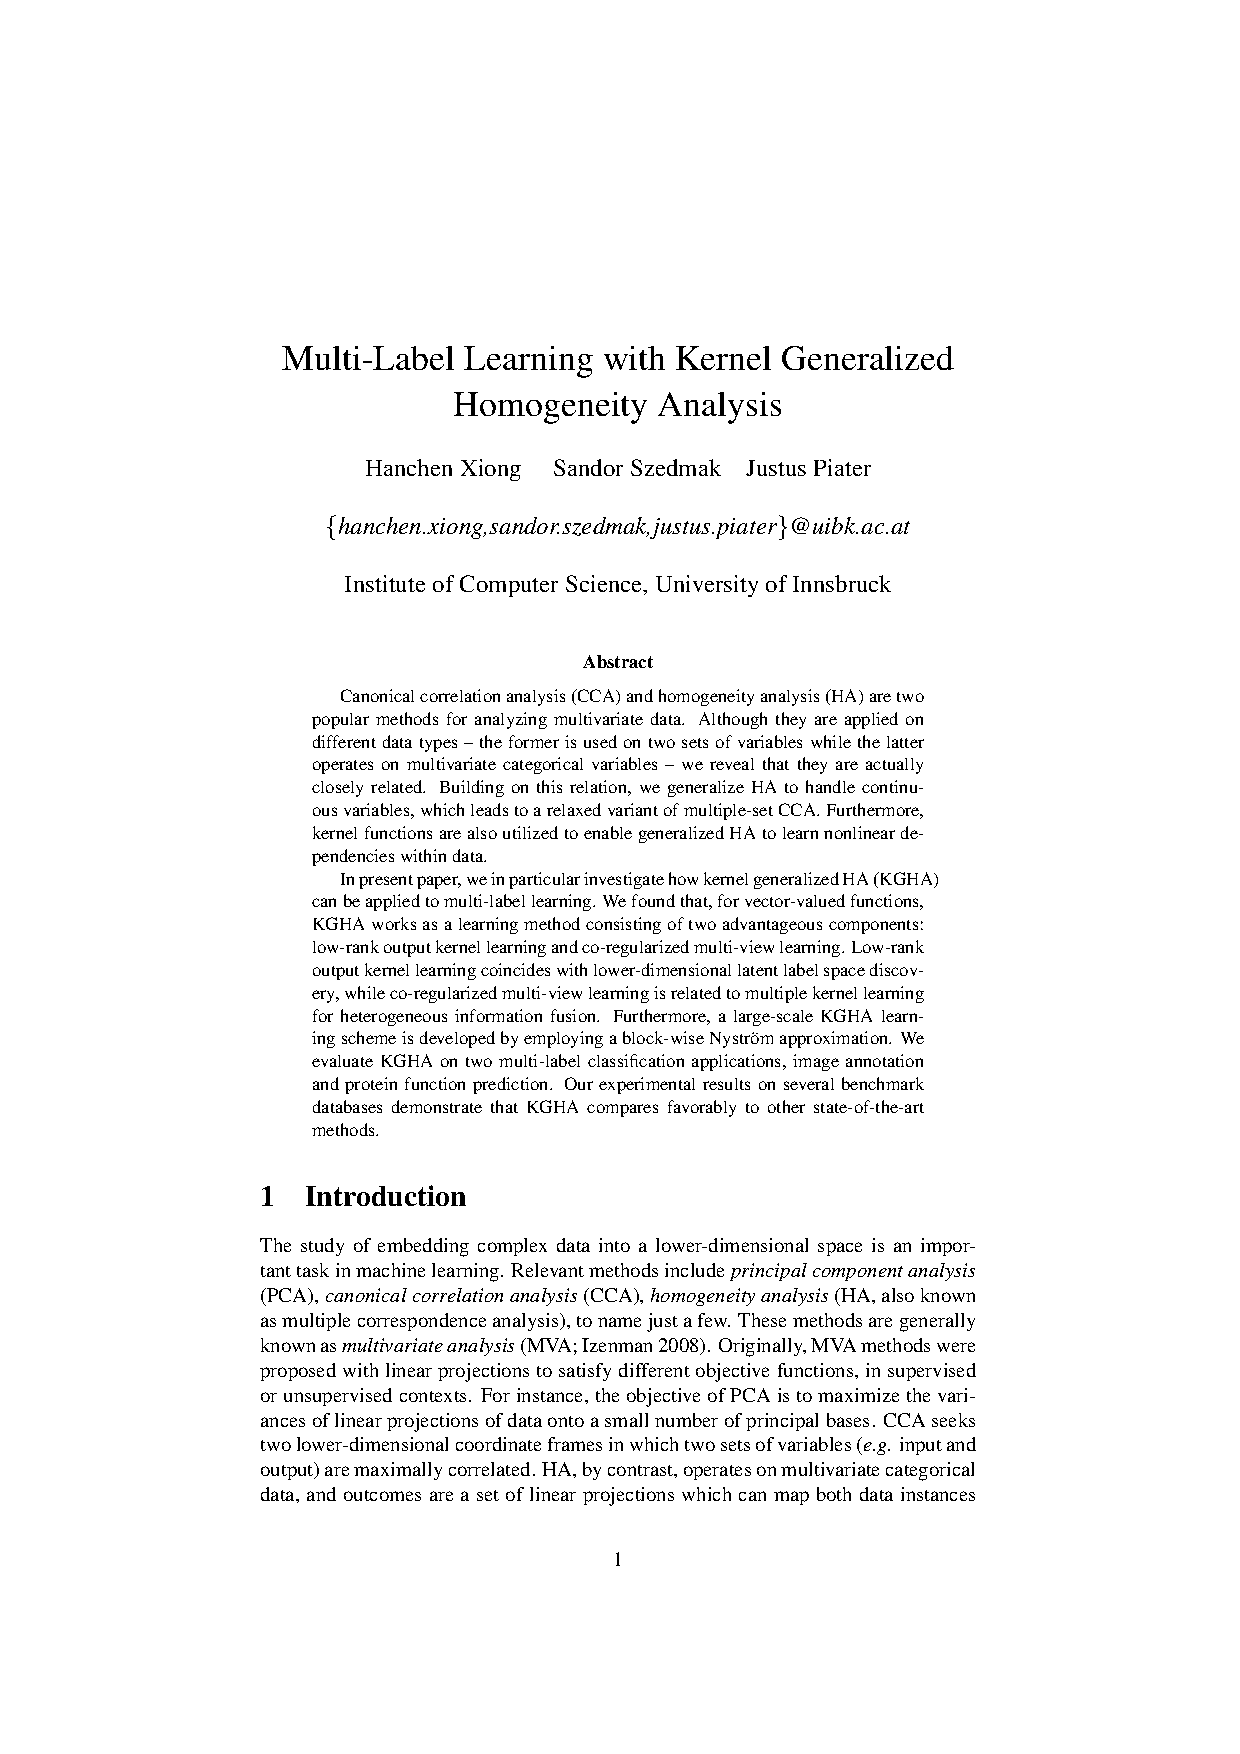
\includepdf[offset=3cm -3cm, scale=1.2, pages=-,pagecommand={\pagestyle{fancy}}]{./Papers/KGHA.pdf}

 
% Chapter Template

\chapter{Optimization on Structures} % Main chapter title
\label{Chapter5} % Change X to a consecutive number; for referencing this chapter elsewhere, use \ref{ChapterX}
\lhead{Chapter 5. \emph{Optimization on Structures}} % Change X to a consecutive number; this is for the header on each page - perhaps a shortened title



\rule{\textwidth}{0.4pt} \\[0.5cm]
\textit{``For the things we have to learn before we can do them, we learn by doing them"}

\begin{flushright}
Aristotle
\end{flushright}
\rule{\textwidth}{0.4pt} 
\newline 
\newline 
This chapter is dedicated to the optimization on structured data. Basically, two forms of structures are considered. First, in section          
\ref{sec:optimize_graph}, optimization on graphical models is studied. Second, in section \ref{sec:optimize_matrix}, structures on 
manifold are considered. More precisely, the optimization on matrix manifolds are studied. 

%----------------------------------------------------------------------------------------
%	SECTION 1
%----------------------------------------------------------------------------------------
\section{Optimization on Graphs}
\label{sec:optimize_graph}
In this section, two optimization methods are reviewed: \emph{max-product (loopy) belief propagation} and \emph{iterated conditional modes} (ICMs).  
Max-product (loopy) belief propagation is an extension of belief propagation inference, which was explained in section \ref{sec:inference}, while 
ICMs is an iterative ``greedy" strategy for local optimization.    
There also exist other notable optimization methods for graphical models, such as \emph{graph cut}, \emph{tree-reweighted message passing}. 
Meanwhile, they are not added in this dissertation. Readers are referred to \cite{many_optimizations} for a review and comparison of them.   



\subsection{Max-product (Loopy) Belief Propagation}
In the belief propagation algorithm (section \ref{sec:inference}), a variable node sends a message to one of its neighbours by first
receiving messages from other neighbours and summing itself out in the product of incoming messages and the occupied potential function.  
Therefore, it is also referred to as \emph{sum-product algorithm} for factor graphs. Optimization actually can be also considered as     
inference by replacing \emph{sum} with \emph{max}, which results in max-product belief propagation, of which the pseudo-code is presented 
in Algorithm \ref{alg:Max_BP_tree}
 \begin{algorithm}
	\caption{Max-product Belief Propagation for tree-structured Markov networks}
	\label{alg:Max_BP_tree}
\begin{algorithmic}[1]
\STATE  select one variable as the root; 
\STATE  starting from all leaves, propagate \emph{beliefs} toward the root as:
\begin{equation*}
m_{i \rightarrow j}(x_j)= \max_{x_i}\left\{\phi(x_i,x_j) \prod_{k\in \text{Ne}(i)\backslash j} m_{k \rightarrow i}(x_i)\right\}
\end{equation*}
\STATE  when the root receives all messages from its neighbors, then propagate backwards the \emph{``inverse beliefs"} as the step 2;
\STATE  the optimization solution of each variable is computed as: 
\begin{equation*}
	x_i=\argmax_{x_i} \prod_{k\in \text{Ne}(i)} m_{k \rightarrow i}(x_i)
\end{equation*}
where Ne$(i)$ denotes the neighboring variables of $x_i$ in the graph. 
\end{algorithmic}
\end{algorithm}

Analogously, the max-product loopy belief propagation can be written out (see Algorithm \ref{alg:max_LBP}) for loopy Markov networks.  
\begin{algorithm}
	\caption{Max-product Loopy Belief Propagation for Loopy Markov networks}
	\label{alg:max_LBP}
\begin{algorithmic}[1]
%\STATE  In a loopy graph, there is no root and leaves because of loop.
\STATE  initialize all messages $m_{i\rightarrow j}$ in both directions of all connected variables randomly or with a constant value (\emph{e.g.} 1);
\WHILE {all messages converge}
\STATE  update messages as:
\begin{equation*}
  m^{(t+1)}_{i \rightarrow j}(x_j)= \max_{x_i}\left\{\phi(x_i,x_j) \prod_{k\in \text{Ne}(i)\backslash j} m^{(t)}_{k \rightarrow i}(x_i)\right\}
\end{equation*}
\ENDWHILE
\end{algorithmic}
\end{algorithm}


\subsection{Iterated Conditional Modes}
Iterated conditional modes (ICMs) is a simple ``greedy" strategy for the optimization of Markov networks. Basically, all variables are initialized randomly and then the state 
of each variable $x_i$ is determined by maximizing the product of all potential functions which involve $x_i$. This state update is iteratively carried out for all variables       
until convergence. 

\section{Optimization on Matrix Manifolds}
\label{sec:optimize_matrix}
In many practical problems, the optimization is with respect to matrices which satisfy certain properties.   
A few examples are enumerated as follow:     
\begin{itemize}
	\item \textbf{Oblique manifold}: $\mathcal{M}=\{X\in\mathbb{R}^{n\times m}: diag (X^\top X)=\mathbf{1}_m \}$; 
	\item \textbf{Stiefel manifold}: $\mathcal{M}=\{X\in\mathbb{R}^{n\times m}: X^\top X=I_m \}$; 
	\item \textbf{SO(n) manifold}: $\mathcal{M}=\{X\in\mathbb{R}^{n\times n}: X^\top X=I_n \text{ and } det(X)=1\}$. 
\end{itemize}
These matrices can also be considered as structures, in which entries are dependent by satisfying different constraints.    
Usually, optimization techniques on matrix manifolds are used to find the optimal matrix. A review of relevant methods      
is provided in \cite{matrix_manifold}.  
In the following subsection, an application of the optimization on the SE(3) manifold on 3D shape registration is presented, which 
shows a representative example of this type of optimization.    

\subsection{3D Point Cloud Registration with Optimization on SE(3) Manifold} 
Despite intensive study, 3D shape
registration remains an open question. 
Here, a novel and efficient registration method is proposed. 
Quite
different from previous registration methods, instead of computing
correspondence and aligning in 3D space, the proposed algorithm first maps 
points to a higher dimensional reproducing  kernel Hilbert space by applying
kernel methods. Registration is subsequently performed within the feature
space by aligning principal components using kernel PCA. The alignment is
projected back into 3D pose space. The whole procedure is
theoretically elegant and efficient. Kernel PCA is used to avoid
explicit computation in feature space, and SE(3) on-manifold
optimization is employed for the convex optimization in the alignment projection. 
Empirical results demonstrate that the proposed method is quite accurate
and robust to various challenging circumstances (\emph{e.g.} large motions,
outliers), and remarkably, it is much faster than other
state-of-the-art methods with comparable performance. 
More technical details and results are presented in the paper IX by the author. 


\begin{shaded}
 {\Huge IX.} \textbf{Hanchen Xiong}, Sandor Szedmak, Justus Piater {\it Efficient, General Point Cloud Registration With Kernel Feature Maps}, 
In Proceedings of 10th International Conference on Computer and Robot Vision (CRV13), pp 83-90, 2013, IEEE.
\end{shaded}
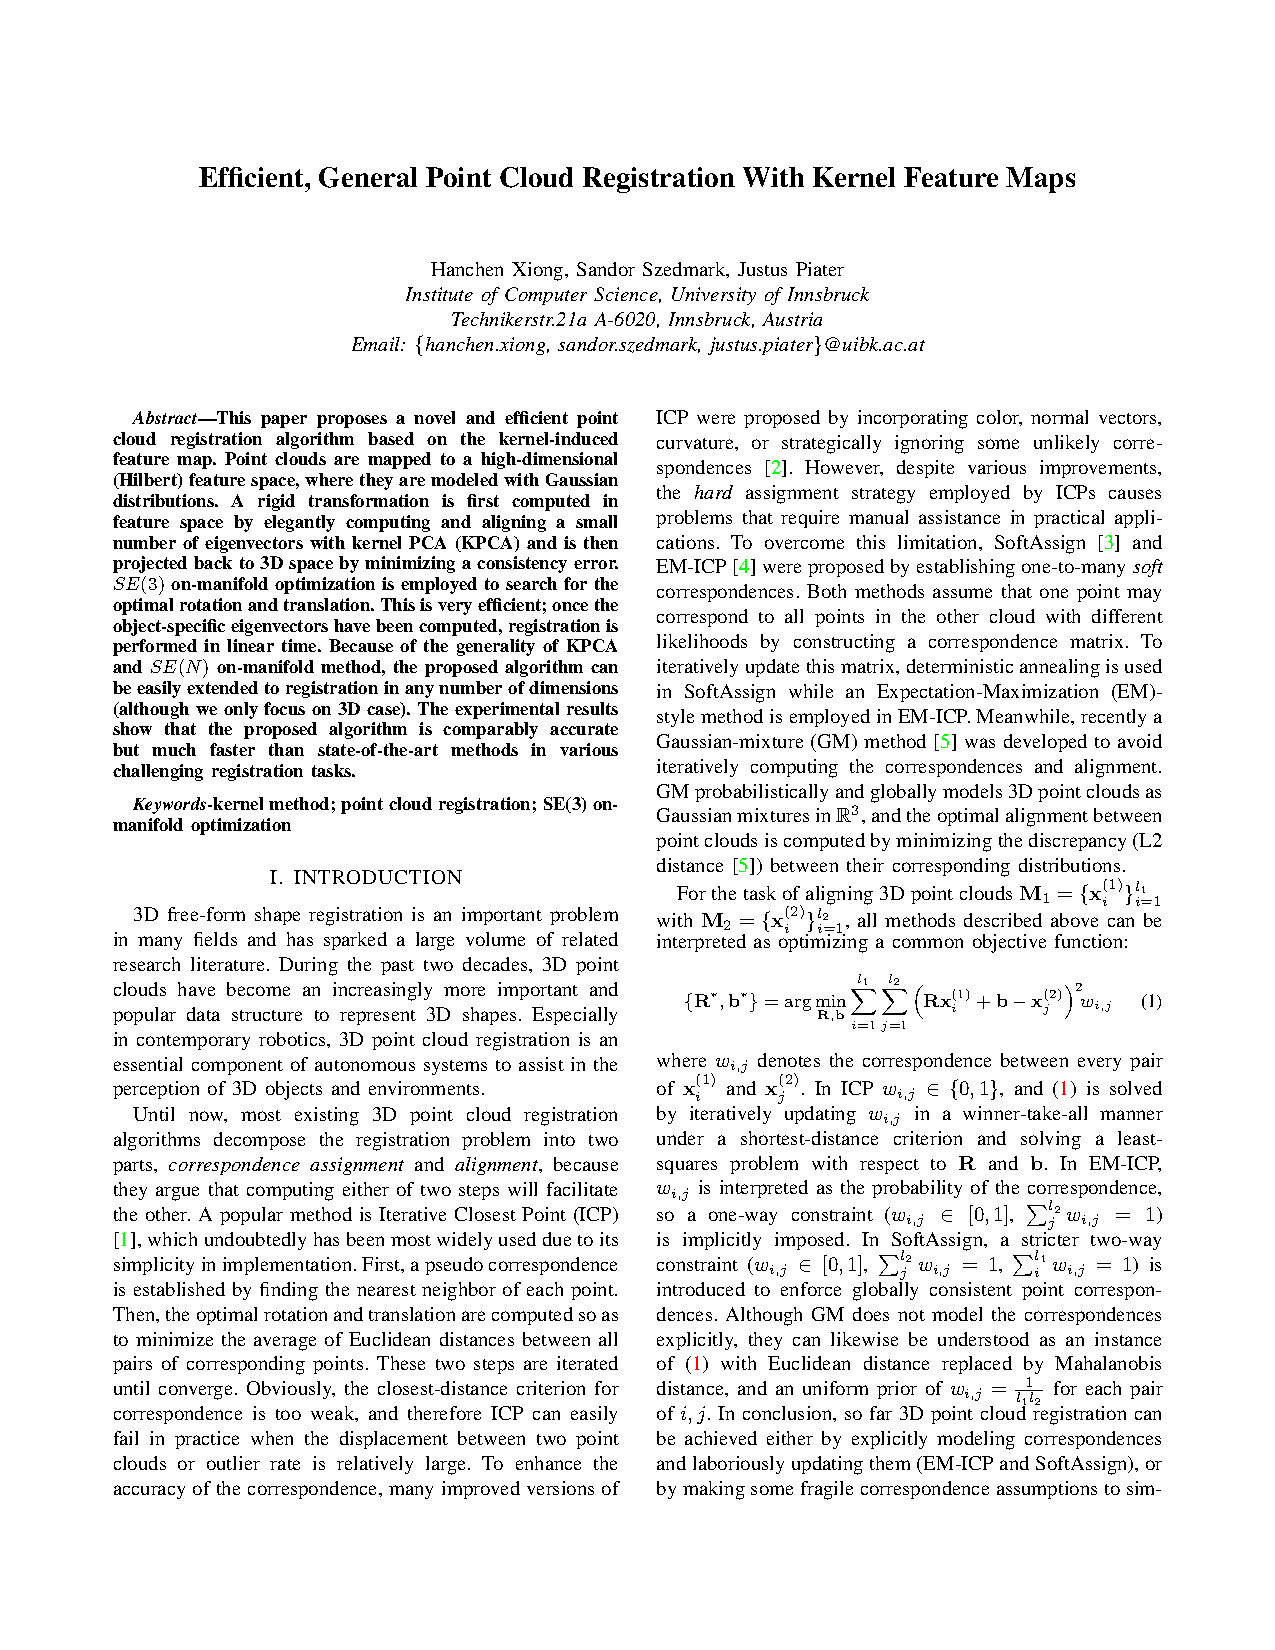
\includepdf[offset=3cm -3cm, scale=1, pages=-,pagecommand={\pagestyle{fancy}}]{./Papers/Xiong-2013-CRV.pdf}


%----------------------------------------------------------------------------------------
%	SECTION 2
%----------------------------------------------------------------------------------------


%\section{Stochastic Optmization of Black-box Functions on Riemannian Manifolds using Kernel Adaptive Sequential Monte Carlo}
%
%Sed ullamcorper quam eu nisl interdum at interdum enim egestas. Aliquam placerat justo sed lectus lobortis ut porta nisl porttitor. Vestibulum mi dolor, lacinia molestie gravida at, tempus vitae ligula. Donec eget quam sapien, in viverra eros. Donec pellentesque justo a massa fringilla non vestibulum metus vestibulum. Vestibulum in orci quis felis tempor lacinia. Vivamus ornare ultrices facilisis. Ut hendrerit volutpat vulputate. Morbi condimentum venenatis augue, id porta ipsum vulputate in. Curabitur luctus tempus justo. Vestibulum risus lectus, adipiscing nec condimentum quis, condimentum nec nisl. Aliquam dictum sagittis velit sed iaculis. Morbi tristique augue sit amet nulla pulvinar id facilisis ligula mollis. Nam elit libero, tincidunt ut aliquam at, molestie in quam. Aenean rhoncus vehicula hendrerit.
%
%
%
 
% Chapter Template

\chapter{Conclusion} % Main chapter title

\label{Chapter6} % Change X to a consecutive number; for referencing this chapter elsewhere, use \ref{ChapterX}

\lhead{Chapter 6. \emph{Conlusion}} % Change X to a consecutive number; this is for the header on each page - perhaps a shortened title

\rule{\textwidth}{0.4pt} \\[0.5cm]
\textit{``The true face of Lushan is lost to my sight, for it is right in this mountain that I reside."}

\begin{flushright}
Su Shi
\end{flushright}
\rule{\textwidth}{0.4pt} 

In previous chapters, structured domains were dealt with different forms and correspondingly computed with different methods.   
The contributions of this dissertation are twofold. The first one is practical, along with a number of experiments on practical tasks, some basic 
principles in the modeling and computation of structured data are illustrated. The second one, however, is relative theoretic, several        
novel models and learning algorithms were proposed, gaining deeper insights into structured-output learning problems.           

After going through four technical chapters, it is useful to step outside and look at the big picture.    
Although the dissertation is organized with three separate parts: inference, learning and optimization, one can be already 
aware of that they are highly connected.                
Some connections can be listed as follows:  
\begin{itemize}
    \item A Bayesian network can be considered as a special case of a Markov network with conditional distributions as its potential functions;        
	\item conditional random fields are related to max-margin Markov networks;
	\item a max-margin Markov network is essentially equivalent to structural SVM;  
	\item joint SVM is a special case of structural SVM on multi-label learning with linear output kernels;        
	\item learning undirected graphical models with maximum likelihood estimation is highly dependent on the inference performance, for example, 
		persistent Sequential Monte Carlo is a learning algorithm based on sampling-based inference;            
	\item optimization of graphical models using max-product (loopy) belief propagation is an extension of (loopy) belief propagation inference.     
\end{itemize}
All connections are also visualized in Figure \ref{fig:conclusion}. It can be seen that working with structured data itself is a 
structure where different topics can interact each other. For example, better inference can improve learning performance while better learning 
can make inference-based prediction more accurate; a good learning method for max-margin Markov networks can be also promising for the structural SVM and 
vice verse.  
\begin{figure}[h]
	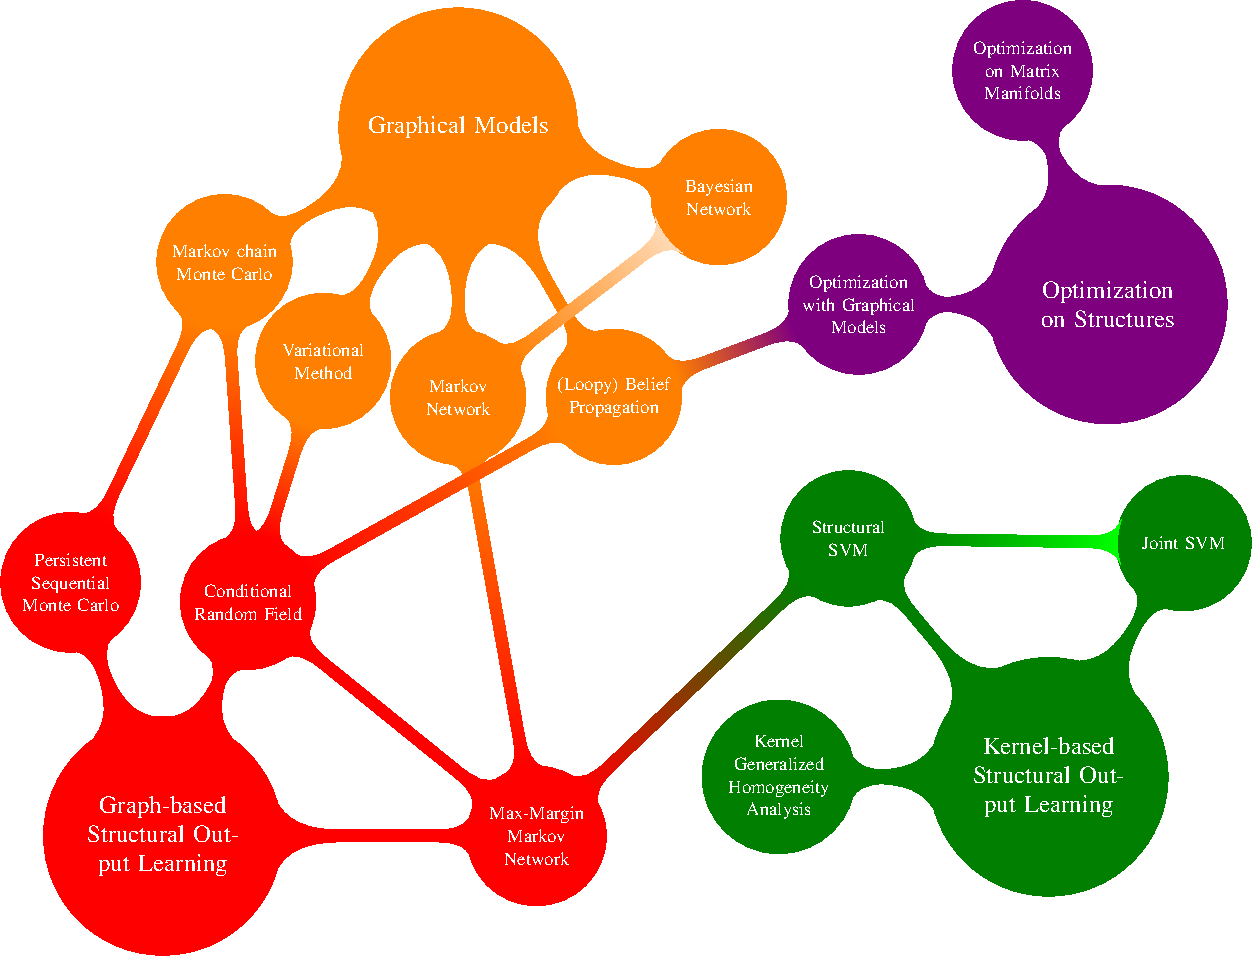
\includegraphics[width=\textwidth]{./Figures/Conclusion_figure-crop}
\caption{How different chapters and sections relate to each other.  }
\label{fig:conclusion}
\end{figure}


Therefore, the main message delivered from the dissertation is to keep a ``structure" mind when confronting multiple data.       
Given a task, based on its nature or characteristic, a structure form is selected and some components in Figure \ref{fig:conclusion} will be involved. 
Furthermore, check how the involved components interact with other ones in the diagram, and then improve the performance by exploiting 
their connections. 

Above all, the content presented in this dissertation is limited. There exist more studies which are influential in relevant       
areas. Also, more developments of working on structured data are expected with increasingly strong desires in practice.        

 
%\input{Chapters/Chapter7} 

%----------------------------------------------------------------------------------------
%	THESIS CONTENT - APPENDICES
%----------------------------------------------------------------------------------------

\addtocontents{toc}{\vspace{2em}} % Add a gap in the Contents, for aesthetics

\appendix % Cue to tell LaTeX that the following 'chapters' are Appendices

% Include the appendices of the thesis as separate files from the Appendices folder
% Uncomment the lines as you write the Appendices

%% Appendix A

\chapter{Appendix Title Here} % Main appendix title

\label{AppendixA} % For referencing this appendix elsewhere, use \ref{AppendixA}

\lhead{Appendix A. \emph{Appendix Title Here}} % This is for the header on each page - perhaps a shortened title

Write your Appendix content here.
%\input{Appendices/AppendixB}
%\input{Appendices/AppendixC}

\addtocontents{toc}{\vspace{2em}} % Add a gap in the Contents, for aesthetics

\backmatter

%----------------------------------------------------------------------------------------
%	BIBLIOGRAPHY
%----------------------------------------------------------------------------------------

\label{Bibliography}

\lhead{\emph{Bibliography}} % Change the page header to say "Bibliography"

\bibliographystyle{plainnat} % Use the "unsrtnat" BibTeX style for formatting the Bibliography
\bibliography{refs} % The references (bibliography) information are stored in the file named "Bibliography.bib"

\end{document}  
